%%____________________________________________________________________________||
\section{Data sets}
\label{sec:datasets}

\subsection{Data}


In this note, we use proton-proton collision data at $\sqrt{s} =$
13~TeV collected in 2015. This version of the note uses 1.2~\ifb of
data certified by the physics validation group. The JSON file listed
in Table~\ref{tab:cert_json} specifies the periods of the time in
which these certified data are collected.
Table~\ref{tab:datasets_data} lists the names of the data sets
relevant for the analysis, along with the integrated luminosities for
each data set. Since the certification of the data collected in 2015
is ongoing, we will use more data in the final version of the note.

We perform a blind analysis. In the previous version of the note, the
data in the signal region is blinded with the exception of 149.48~\ipb
of the certified data specified by the JSON file in
Table~\ref{tab:cert_unblind_json}. Data in the control regions is
never blinded. These bliding policies are agree in the SUS PAG.

In the review of the previous version of the note and related
presentations in the SUS PAG, it becomes clear that we understand the
data in the control regions and a small fraction of the unblinded data
in the signal region well enough to predict the backgrounds in the
signal region. As a result, no data in the signal region is blinded in
this version of the note.

\begin{table}[!h]
\topcaption{The JSON file that specifies the periods of the time in
which 1.2~\ifb of the certified data are collected} \footnotesize
%latex.default(d, title = NULL, booktabs = FALSE, width = 3, rowname = NULL,     helvetica = FALSE, caption.loc = "bottom", ...)%
\begin{center}
\begin{tabular}{c}
\hline\hline
\verb!Cert_271036-276811_13TeV_PromptReco_Collisions16_JSON.txt!\tabularnewline
\hline
\end{tabular}\end{center}
 \label{tab:cert_json}
\end{table}

\begin{table}[!h]
\topcaption{Data sets}
\footnotesize \begin{center}
\begin{tabular}{l}
\hline\hline
\multicolumn{1}{c}{Data set}\tabularnewline
\hline
\verb!/HTMHT/Run2016B-23Sep2016-v3/MINIAOD!\tabularnewline
\verb!/HTMHT/Run2016C-23Sep2016-v1/MINIAOD!\tabularnewline
\verb!/HTMHT/Run2016D-23Sep2016-v1/MINIAOD!\tabularnewline
\verb!/HTMHT/Run2016E-23Sep2016-v1/MINIAOD!\tabularnewline
\verb!/HTMHT/Run2016F-23Sep2016-v1/MINIAOD!\tabularnewline
\verb!/HTMHT/Run2016G-23Sep2016-v2/MINIAOD!\tabularnewline
\verb!/HTMHT/Run2016H-PromptReco-v2/MINIAOD!\tabularnewline
\verb!/HTMHT/Run2016H-PromptReco-v3/MINIAOD!\tabularnewline
\verb!/JetHT/Run2016B-23Sep2016-v2/MINIAOD!\tabularnewline
\verb!/JetHT/Run2016C-23Sep2016-v2/MINIAOD!\tabularnewline
\verb!/JetHT/Run2016D-23Sep2016-v2/MINIAOD!\tabularnewline
\verb!/JetHT/Run2016E-23Sep2016-v1/MINIAOD!\tabularnewline
\verb!/JetHT/Run2016F-23Sep2016-v1/MINIAOD!\tabularnewline
\verb!/JetHT/Run2016G-23Sep2016-v2/MINIAOD!\tabularnewline
\verb!/JetHT/Run2016H-PromptReco-v2/MINIAOD!\tabularnewline
\verb!/JetHT/Run2016H-PromptReco-v3/MINIAOD!\tabularnewline
\verb!/MET/Run2016B-23Sep2016-v3/MINIAOD!\tabularnewline
\verb!/MET/Run2016C-23Sep2016-v1/MINIAOD!\tabularnewline
\verb!/MET/Run2016D-23Sep2016-v1/MINIAOD!\tabularnewline
\verb!/MET/Run2016E-23Sep2016-v1/MINIAOD!\tabularnewline
\verb!/MET/Run2016F-23Sep2016-v1/MINIAOD!\tabularnewline
\verb!/MET/Run2016G-23Sep2016-v1/MINIAOD!\tabularnewline
\verb!/MET/Run2016H-PromptReco-v2/MINIAOD!\tabularnewline
\verb!/SingleMuon/Run2016B-23Sep2016-v3/MINIAOD!\tabularnewline
\verb!/SingleMuon/Run2016C-23Sep2016-v1/MINIAOD!\tabularnewline
\verb!/SingleMuon/Run2016D-23Sep2016-v1/MINIAOD!\tabularnewline
\verb!/SingleMuon/Run2016E-23Sep2016-v1/MINIAOD!\tabularnewline
\verb!/SingleMuon/Run2016F-23Sep2016-v1/MINIAOD!\tabularnewline
\verb!/SingleMuon/Run2016G-23Sep2016-v1/MINIAOD!\tabularnewline
\verb!/SingleMuon/Run2016H-PromptReco-v2/MINIAOD!\tabularnewline
\verb!/SingleMuon/Run2016H-PromptReco-v3/MINIAOD!\tabularnewline
\verb!/SinglePhoton/Run2016B-23Sep2016-v3/MINIAOD!\tabularnewline
\verb!/SinglePhoton/Run2016C-23Sep2016-v1/MINIAOD!\tabularnewline
\verb!/SinglePhoton/Run2016D-23Sep2016-v1/MINIAOD!\tabularnewline
\verb!/SinglePhoton/Run2016E-23Sep2016-v1/MINIAOD!\tabularnewline
\verb!/SinglePhoton/Run2016F-23Sep2016-v1/MINIAOD!\tabularnewline
\verb!/SinglePhoton/Run2016G-23Sep2016-v1/MINIAOD!\tabularnewline
\verb!/SinglePhoton/Run2016H-PromptReco-v2/MINIAOD!\tabularnewline
\verb!/SinglePhoton/Run2016H-PromptReco-v3/MINIAOD!\tabularnewline
\verb!/DoubleEG/Run2016B-23Sep2016-v3/MINIAOD!\tabularnewline
\verb!/DoubleEG/Run2016C-23Sep2016-v1/MINIAOD!\tabularnewline
\verb!/DoubleEG/Run2016D-23Sep2016-v1/MINIAOD!\tabularnewline
\verb!/DoubleEG/Run2016E-23Sep2016-v1/MINIAOD!\tabularnewline
\verb!/DoubleEG/Run2016F-23Sep2016-v1/MINIAOD!\tabularnewline
\verb!/DoubleEG/Run2016G-23Sep2016-v1/MINIAOD!\tabularnewline
\verb!/DoubleEG/Run2016H-PromptReco-v2/MINIAOD!\tabularnewline
\verb!/DoubleEG/Run2016H-PromptReco-v3/MINIAOD!\tabularnewline
\hline
\end{tabular}\end{center}

\label{tab:datasets_data}
\end{table}

\begin{table}[!h]
\topcaption{The JSON file specifying the 149.48~\ipb of the certified
data that we never blind} \footnotesize
%latex.default(d, title = NULL, booktabs = FALSE, width = 3, rowname = NULL,     helvetica = FALSE, caption.loc = "bottom", ...)%
\begin{center}
\begin{tabular}{c}
\hline\hline
 \verb!Cert_246908-257599_13TeV_PromptReco_Collisions15_25ns_JSON_v3.txt!\tabularnewline
\hline
\end{tabular}\end{center}

\label{tab:cert_unblind_json}
\end{table}

\subsection{Simulation}

Table~\ref{tab:datasets_bkg} lists the data sets of simulated events
of the standard model background processes used in this note. In these
data sets, in addition to the main interaction, each event contains on
average 20 minimum bias interactions which simulate multiple
interactions per bunch-crossing (in-time pileup). The expected detector
signal from previous or following bunch crossings (out-of-time pileup)
with 25ns bunch spacing is overlapped.

 \begin{table}[!h]
  \centering
  \topcaption{Simulated background samples}
  \scriptsize
  \scalebox{.7}[1.0]{%latex.default(d, title = NULL, booktabs = FALSE, width = 3, rowname = NULL,     helvetica = FALSE, caption.loc = "bottom", ...)%
\begin{center}
\begin{tabular}{ll}
\hline\hline
\multicolumn{1}{c}{Data set}&\multicolumn{1}{c}{Cross section [pb]}\tabularnewline
\hline
\verb!/DYJetsToLL_M-10to50_TuneCUETP8M1_13TeV-amcatnloFXFX-pythia8/RunIISpring15DR74-Asympt25ns_MCRUN2_74_V9-v1/MINIAODSIM! &$1.861\times 10^{+04}$\tabularnewline
\verb!/DYJetsToLL_M-50_TuneCUETP8M1_13TeV-amcatnloFXFX-pythia8/RunIISpring15DR74-Asympt25ns_MCRUN2_74_V9-v3/MINIAODSIM! &$6.024\times 10^{+03}$\tabularnewline
\verb!/DYJetsToLL_M-50_HT-100to200_TuneCUETP8M1_13TeV-madgraphMLM-pythia8/RunIISpring15DR74-Asympt25ns_MCRUN2_74_V9-v2/MINIAODSIM! &$1.715\times 10^{+02}$\tabularnewline
\verb!/DYJetsToLL_M-50_HT-200to400_TuneCUETP8M1_13TeV-madgraphMLM-pythia8/RunIISpring15DR74-Asympt25ns_MCRUN2_74_V9-v2/MINIAODSIM! &$5.258\times 10^{+01}$\tabularnewline
\verb!/DYJetsToLL_M-50_HT-400to600_TuneCUETP8M1_13TeV-madgraphMLM-pythia8/RunIISpring15DR74-Asympt25ns_MCRUN2_74_V9-v2/MINIAODSIM! &$6.761\times 10^{+00}$\tabularnewline
\verb!/DYJetsToLL_M-50_HT-600toInf_TuneCUETP8M1_13TeV-madgraphMLM-pythia8/RunIISpring15DR74-Asympt25ns_MCRUN2_74_V9-v2/MINIAODSIM! &$2.718\times 10^{+00}$\tabularnewline
\verb!/GJets_HT-40To100_TuneCUETP8M1_13TeV-madgraphMLM-pythia8/RunIISpring15DR74-Asympt25ns_MCRUN2_74_V9-v2/MINIAODSIM! &$2.308\times 10^{+04}$\tabularnewline
\verb!/GJets_HT-100To200_TuneCUETP8M1_13TeV-madgraphMLM-pythia8/RunIISpring15DR74-Asympt25ns_MCRUN2_74_V9-v2/MINIAODSIM! &$9.110\times 10^{+03}$\tabularnewline
\verb!/GJets_HT-200To400_TuneCUETP8M1_13TeV-madgraphMLM-pythia8/RunIISpring15DR74-Asympt25ns_MCRUN2_74_V9-v2/MINIAODSIM! &$2.298\times 10^{+03}$\tabularnewline
\verb!/GJets_HT-400To600_TuneCUETP8M1_13TeV-madgraphMLM-pythia8/RunIISpring15DR74-Asympt25ns_MCRUN2_74_V9-v1/MINIAODSIM! &$2.730\times 10^{+02}$\tabularnewline
\verb!/GJets_HT-600ToInf_TuneCUETP8M1_13TeV-madgraphMLM-pythia8/RunIISpring15DR74-Asympt25ns_MCRUN2_74_V9-v1/MINIAODSIM! &$9.450\times 10^{+01}$\tabularnewline
\verb!/QCD_HT100to200_TuneCUETP8M1_13TeV-madgraphMLM-pythia8/RunIISpring15DR74-Asympt25ns_MCRUN2_74_V9-v2/MINIAODSIM! &$2.754\times 10^{+07}$\tabularnewline
\verb!/QCD_HT200to300_TuneCUETP8M1_13TeV-madgraphMLM-pythia8/RunIISpring15DR74-Asympt25ns_MCRUN2_74_V9-v2/MINIAODSIM! &$1.735\times 10^{+06}$\tabularnewline
\verb!/QCD_HT300to500_TuneCUETP8M1_13TeV-madgraphMLM-pythia8/RunIISpring15DR74-Asympt25ns_MCRUN2_74_V9-v2/MINIAODSIM! &$3.670\times 10^{+05}$\tabularnewline
\verb!/QCD_HT500to700_TuneCUETP8M1_13TeV-madgraphMLM-pythia8/RunIISpring15DR74-Asympt25ns_MCRUN2_74_V9-v1/MINIAODSIM! &$2.940\times 10^{+04}$\tabularnewline
\verb!/QCD_HT700to1000_TuneCUETP8M1_13TeV-madgraphMLM-pythia8/RunIISpring15DR74-Asympt25ns_MCRUN2_74_V9-v1/MINIAODSIM! &$6.524\times 10^{+03}$\tabularnewline
\verb!/QCD_HT1000to1500_TuneCUETP8M1_13TeV-madgraphMLM-pythia8/RunIISpring15DR74-Asympt25ns_MCRUN2_74_V9-v2/MINIAODSIM! &$1.064\times 10^{+03}$\tabularnewline
\verb!/QCD_HT1500to2000_TuneCUETP8M1_13TeV-madgraphMLM-pythia8/RunIISpring15DR74-Asympt25ns_MCRUN2_74_V9-v1/MINIAODSIM! &$1.215\times 10^{+02}$\tabularnewline
\verb!/QCD_HT2000toInf_TuneCUETP8M1_13TeV-madgraphMLM-pythia8/RunIISpring15DR74-Asympt25ns_MCRUN2_74_V9-v1/MINIAODSIM! &$2.542\times 10^{+01}$\tabularnewline
\verb!/QCD_Pt_80to120_TuneCUETP8M1_13TeV_pythia8/RunIISpring15DR74-Asympt25ns_MCRUN2_74_V9-v1/MINIAODSIM! &$2.763\times 10^{+06}$\tabularnewline
\verb!/QCD_Pt_120to170_TuneCUETP8M1_13TeV_pythia8/RunIISpring15DR74-Asympt25ns_MCRUN2_74_V9-v1/MINIAODSIM! &$4.711\times 10^{+05}$\tabularnewline
\verb!/QCD_Pt_170to300_TuneCUETP8M1_13TeV_pythia8/RunIISpring15DR74-Asympt25ns_MCRUN2_74_V9-v2/MINIAODSIM! &$1.173\times 10^{+05}$\tabularnewline
\verb!/QCD_Pt_300to470_TuneCUETP8M1_13TeV_pythia8/RunIISpring15DR74-Asympt25ns_MCRUN2_74_V9-v1/MINIAODSIM! &$7.823\times 10^{+03}$\tabularnewline
\verb!/QCD_Pt_470to600_TuneCUETP8M1_13TeV_pythia8/RunIISpring15DR74-Asympt25ns_MCRUN2_74_V9-v2/MINIAODSIM! &$6.482\times 10^{+02}$\tabularnewline
\verb!/QCD_Pt_600to800_TuneCUETP8M1_13TeV_pythia8/RunIISpring15DR74-Asympt25ns_MCRUN2_74_V9-v2/MINIAODSIM! &$1.869\times 10^{+02}$\tabularnewline
\verb!/QCD_Pt_800to1000_TuneCUETP8M1_13TeV_pythia8/RunIISpring15DR74-Asympt25ns_MCRUN2_74_V9-v2/MINIAODSIM! &$3.229\times 10^{+01}$\tabularnewline
\verb!/QCD_Pt_1000to1400_TuneCUETP8M1_13TeV_pythia8/RunIISpring15DR74-Asympt25ns_MCRUN2_74_V9-v1/MINIAODSIM! &$9.418\times 10^{+00}$\tabularnewline
\verb!/QCD_Pt_1400to1800_TuneCUETP8M1_13TeV_pythia8/RunIISpring15DR74-Asympt25ns_MCRUN2_74_V9-v1/MINIAODSIM! &$8.427\times 10^{-01}$\tabularnewline
\verb!/QCD_Pt_1800to2400_TuneCUETP8M1_13TeV_pythia8/RunIISpring15DR74-Asympt25ns_MCRUN2_74_V9-v1/MINIAODSIM! &$1.149\times 10^{-01}$\tabularnewline
\verb!/QCD_Pt_2400to3200_TuneCUETP8M1_13TeV_pythia8/RunIISpring15DR74-Asympt25ns_MCRUN2_74_V9-v1/MINIAODSIM! &$6.830\times 10^{-03}$\tabularnewline
\verb!/QCD_Pt_3200toInf_TuneCUETP8M1_13TeV_pythia8/RunIISpring15DR74-Asympt25ns_MCRUN2_74_V9-v1/MINIAODSIM! &$1.654\times 10^{-04}$\tabularnewline
\verb!/ST_tW_antitop_5f_inclusiveDecays_13TeV-powheg-pythia8_TuneCUETP8M1/RunIISpring15DR74-Asympt25ns_MCRUN2_74_V9-v1/MINIAODSIM! &$3.560\times 10^{+01}$\tabularnewline
\verb!/TTJets_TuneCUETP8M1_13TeV-amcatnloFXFX-pythia8/RunIISpring15DR74-Asympt25ns_MCRUN2_74_V9-v1/MINIAODSIM! &$8.318\times 10^{+02}$\tabularnewline
\verb!/TTJets_TuneCUETP8M1_13TeV-madgraphMLM-pythia8/RunIISpring15DR74-Asympt25ns_MCRUN2_74_V9-v2/MINIAODSIM! &$8.318\times 10^{+02}$\tabularnewline
\verb!/ST_s-channel_4f_leptonDecays_13TeV-amcatnlo-pythia8_TuneCUETP8M1/RunIISpring15DR74-Asympt25ns_MCRUN2_74_V9-v1/MINIAODSIM! &$3.681\times 10^{+00}$\tabularnewline
\verb!/ST_t-channel_4f_leptonDecays_13TeV-amcatnlo-pythia8_TuneCUETP8M1/RunIISpring15DR74-Asympt25ns_MCRUN2_74_V9-v1/MINIAODSIM! &$7.031\times 10^{+01}$\tabularnewline
\verb!/ST_tW_top_5f_inclusiveDecays_13TeV-powheg-pythia8_TuneCUETP8M1/RunIISpring15DR74-Asympt25ns_MCRUN2_74_V9-v1/MINIAODSIM! &$3.560\times 10^{+01}$\tabularnewline
\verb!/WJetsToLNu_TuneCUETP8M1_13TeV-amcatnloFXFX-pythia8/RunIISpring15DR74-Asympt25ns_MCRUN2_74_V9-v1/MINIAODSIM! &$6.153\times 10^{+04}$\tabularnewline
\verb!/WJetsToLNu_HT-100To200_TuneCUETP8M1_13TeV-madgraphMLM-pythia8/RunIISpring15DR74-Asympt25ns_MCRUN2_74_V9-v1/MINIAODSIM! &$1.630\times 10^{+03}$\tabularnewline
\verb!/WJetsToLNu_HT-200To400_TuneCUETP8M1_13TeV-madgraphMLM-pythia8/RunIISpring15DR74-Asympt25ns_MCRUN2_74_V9-v1/MINIAODSIM! &$4.356\times 10^{+02}$\tabularnewline
\verb!/WJetsToLNu_HT-400To600_TuneCUETP8M1_13TeV-madgraphMLM-pythia8/RunIISpring15DR74-Asympt25ns_MCRUN2_74_V9-v3/MINIAODSIM! &$5.917\times 10^{+01}$\tabularnewline
\verb!/WJetsToLNu_HT-600To800_TuneCUETP8M1_13TeV-madgraphMLM-pythia8/RunIISpring15DR74-Asympt25ns_MCRUN2_74_V9-v2/MINIAODSIM! &$1.549\times 10^{+01}$\tabularnewline
\verb!/WJetsToLNu_HT-800To1200_TuneCUETP8M1_13TeV-madgraphMLM-pythia8/RunIISpring15DR74-Asympt25ns_MCRUN2_74_V9-v1/MINIAODSIM! &$6.365\times 10^{+00}$\tabularnewline
\verb!/WJetsToLNu_HT-1200To2500_TuneCUETP8M1_13TeV-madgraphMLM-pythia8/RunIISpring15DR74-Asympt25ns_MCRUN2_74_V9-v1/MINIAODSIM! &$1.609\times 10^{+00}$\tabularnewline
\verb!/WJetsToLNu_HT-2500ToInf_TuneCUETP8M1_13TeV-madgraphMLM-pythia8/RunIISpring15DR74-Asympt25ns_MCRUN2_74_V9-v2/MINIAODSIM! &$3.738\times 10^{-02}$\tabularnewline
\verb!/WWTo2L2Nu_13TeV-powheg/RunIISpring15DR74-Asympt25ns_MCRUN2_74_V9-v1/MINIAODSIM! &$1.246\times 10^{+01}$\tabularnewline
\verb!/WZ_TuneCUETP8M1_13TeV-pythia8/RunIISpring15DR74-Asympt25ns_MCRUN2_74_V9-v1/MINIAODSIM! &$6.610\times 10^{+01}$\tabularnewline
\verb!/ZJetsToNuNu_HT-100To200_13TeV-madgraph/RunIISpring15DR74-Asympt25ns_MCRUN2_74_V9-v1/MINIAODSIM! &$3.450\times 10^{+02}$\tabularnewline
\verb!/ZJetsToNuNu_HT-200To400_13TeV-madgraph/RunIISpring15DR74-Asympt25ns_MCRUN2_74_V9-v1/MINIAODSIM! &$9.638\times 10^{+01}$\tabularnewline
\verb!/ZJetsToNuNu_HT-400To600_13TeV-madgraph/RunIISpring15DR74-Asympt25ns_MCRUN2_74_V9-v1/MINIAODSIM! &$1.346\times 10^{+01}$\tabularnewline
\verb!/ZJetsToNuNu_HT-600ToInf_13TeV-madgraph/RunIISpring15DR74-Asympt25ns_MCRUN2_74_V9-v1/MINIAODSIM! &$5.170\times 10^{+00}$\tabularnewline
\verb!/ZZ_TuneCUETP8M1_13TeV-pythia8/RunIISpring15DR74-Asympt25ns_MCRUN2_74_V9-v3/MINIAODSIM! &$3.180\times 10^{+01}$\tabularnewline
\hline
\end{tabular}\end{center}
}
  \label{tab:datasets_bkg}
 \end{table}
\end{landscape}

\begin{table}[!p]
 \centering
 \topcaption{Simulated samples}
 \scriptsize
 \scalebox{.7}[1.0]{%latex.default(d, title = NULL, booktabs = FALSE, width = 3, rowname = NULL,     helvetica = FALSE, caption.loc = "bottom", ...)%
\begin{center}
\begin{tabular}{l}
\hline\hline
\multicolumn{1}{c}{Data set}\tabularnewline
\hline
\verb!/SMS-T1qqqq_mGluino-600_mLSP-1to300_TuneCUETP8M1_13TeV-madgraphMLM-pythia8/RunIISpring15FSPremix-MCRUN2_74_V9-v1/MINIAODSIM! \tabularnewline
\verb!/SMS-T1qqqq_mGluino-600_mLSP-400to475_TuneCUETP8M1_13TeV-madgraphMLM-pythia8/RunIISpring15FSPremix-MCRUN2_74_V9-v1/MINIAODSIM! \tabularnewline
\verb!/SMS-T1qqqq_mGluino-600_mLSP-500to575_TuneCUETP8M1_13TeV-madgraphMLM-pythia8/RunIISpring15FSPremix-MCRUN2_74_V9-v1/MINIAODSIM! \tabularnewline
\verb!/SMS-T1qqqq_mGluino-625_mLSP-425to525_TuneCUETP8M1_13TeV-madgraphMLM-pythia8/RunIISpring15FSPremix-MCRUN2_74_V9-v1/MINIAODSIM! \tabularnewline
\verb!/SMS-T1qqqq_mGluino-625to650_mLSP-475to550_TuneCUETP8M1_13TeV-madgraphMLM-pythia8/RunIISpring15FSPremix-MCRUN2_74_V9-v1/MINIAODSIM! \tabularnewline
\verb!/SMS-T1qqqq_mGluino-675_mLSP-500to650_TuneCUETP8M1_13TeV-madgraphMLM-pythia8/RunIISpring15FSPremix-MCRUN2_74_V9-v1/MINIAODSIM! \tabularnewline
\verb!/SMS-T1qqqq_mGluino-750to775_mLSP-450to750_TuneCUETP8M1_13TeV-madgraphMLM-pythia8/RunIISpring15FSPremix-MCRUN2_74_V9-v1/MINIAODSIM! \tabularnewline
\verb!/SMS-T1qqqq_mGluino-800to825_mLSP-1to750_TuneCUETP8M1_13TeV-madgraphMLM-pythia8/RunIISpring15FSPremix-MCRUN2_74_V9-v1/MINIAODSIM! \tabularnewline
\verb!/SMS-T1qqqq_mGluino-825to875_mLSP-400to825_TuneCUETP8M1_13TeV-madgraphMLM-pythia8/RunIISpring15FSPremix-MCRUN2_74_V9-v1/MINIAODSIM! \tabularnewline
\verb!/SMS-T1qqqq_mGluino-1000to1025_mLSP-1to1000_TuneCUETP8M1_13TeV-madgraphMLM-pythia8/RunIISpring15FSPremix-MCRUN2_74_V9-v1/MINIAODSIM! \tabularnewline
\verb!/SMS-T1qqqq_mGluino-1025to1075_mLSP-400to1050_TuneCUETP8M1_13TeV-madgraphMLM-pythia8/RunIISpring15FSPremix-MCRUN2_74_V9-v1/MINIAODSIM! \tabularnewline
\verb!/SMS-T1qqqq_mGluino-1075_mLSP-925to975_TuneCUETP8M1_13TeV-madgraphMLM-pythia8/RunIISpring15FSPremix-MCRUN2_74_V9-v1/MINIAODSIM! \tabularnewline
\verb!/SMS-T1qqqq_mGluino-1100to1125_mLSP-1to1100_TuneCUETP8M1_13TeV-madgraphMLM-pythia8/RunIISpring15FSPremix-MCRUN2_74_V9-v1/MINIAODSIM! \tabularnewline
\verb!/SMS-T1qqqq_mGluino-1125to1175_mLSP-925to1125_TuneCUETP8M1_13TeV-madgraphMLM-pythia8/RunIISpring15FSPremix-MCRUN2_74_V9-v1/MINIAODSIM! \tabularnewline
\verb!/SMS-T1qqqq_mGluino-1225to1250_mLSP-1to1225_TuneCUETP8M1_13TeV-madgraphMLM-pythia8/RunIISpring15FSPremix-MCRUN2_74_V9-v1/MINIAODSIM! \tabularnewline
\verb!/SMS-T1qqqq_mGluino-1250to1275_mLSP-550to1250_TuneCUETP8M1_13TeV-madgraphMLM-pythia8/RunIISpring15FSPremix-MCRUN2_74_V9-v1/MINIAODSIM! \tabularnewline
\verb!/SMS-T1qqqq_mGluino-1300to1325_mLSP-1to1275_TuneCUETP8M1_13TeV-madgraphMLM-pythia8/RunIISpring15FSPremix-MCRUN2_74_V9-v1/MINIAODSIM! \tabularnewline
\verb!/SMS-T1qqqq_mGluino-1325to1350_mLSP-1to1275_TuneCUETP8M1_13TeV-madgraphMLM-pythia8/RunIISpring15FSPremix-MCRUN2_74_V9-v1/MINIAODSIM! \tabularnewline
\verb!/SMS-T1qqqq_mGluino-1400to1450_mLSP-1to1275_TuneCUETP8M1_13TeV-madgraphMLM-pythia8/RunIISpring15FSPremix-MCRUN2_74_V9-v1/MINIAODSIM! \tabularnewline
\verb!/SMS-T1qqqq_mGluino-1450to1500_mLSP-1to1275_TuneCUETP8M1_13TeV-madgraphMLM-pythia8/RunIISpring15FSPremix-MCRUN2_74_V9-v1/MINIAODSIM! \tabularnewline
\verb!/SMS-T1qqqq_mGluino-1500to1550_mLSP-1to1250_TuneCUETP8M1_13TeV-madgraphMLM-pythia8/RunIISpring15FSPremix-MCRUN2_74_V9-v1/MINIAODSIM! \tabularnewline
\verb!/SMS-T1qqqq_mGluino-1550_mLSP-950_TuneCUETP8M1_13TeV-madgraphMLM-pythia8/RunIISpring15FSPremix-MCRUN2_74_V9-v1/MINIAODSIM! \tabularnewline
\verb!/SMS-T1qqqq_mGluino-1600to1650_mLSP-1to1250_TuneCUETP8M1_13TeV-madgraphMLM-pythia8/RunIISpring15FSPremix-MCRUN2_74_V9-v1/MINIAODSIM! \tabularnewline
\verb!/SMS-T1qqqq_mGluino-1650to1750_mLSP-1to1250_TuneCUETP8M1_13TeV-madgraphMLM-pythia8/RunIISpring15FSPremix-MCRUN2_74_V9-v1/MINIAODSIM! \tabularnewline
\verb!/SMS-T1qqqq_mGluino-1750_mLSP-50to1250_TuneCUETP8M1_13TeV-madgraphMLM-pythia8/RunIISpring15FSPremix-MCRUN2_74_V9-v1/MINIAODSIM! \tabularnewline
\verb!/SMS-T1qqqq_mGluino-1850to1950_mLSP-1to1250_TuneCUETP8M1_13TeV-madgraphMLM-pythia8/RunIISpring15FSPremix-MCRUN2_74_V9-v1/MINIAODSIM! \tabularnewline
\verb!/SMS-T1qqqq_mGluino-1950to2000_mLSP-1to1250_TuneCUETP8M1_13TeV-madgraphMLM-pythia8/RunIISpring15FSPremix-MCRUN2_74_V9-v1/MINIAODSIM! \tabularnewline
\verb!/SMS-T1qqqq_mGluino-2000_mLSP-50to950_TuneCUETP8M1_13TeV-madgraphMLM-pythia8/RunIISpring15FSPremix-MCRUN2_74_V9-v1/MINIAODSIM! \tabularnewline
\hline
\end{tabular}\end{center}
}
%\label{tab:datasets_bkg}
\end{table}

\begin{table}[!p]
 \centering
\topcaption{Simulated samples}
 \scriptsize
 \scalebox{.7}[1.0]{%latex.default(d, title = NULL, booktabs = FALSE, width = 3, rowname = NULL,     helvetica = FALSE, caption.loc = "bottom", ...)%
\begin{center}
\begin{tabular}{l}
\hline\hline
\multicolumn{1}{c}{Data set}\tabularnewline
\hline
\verb!/SMS-T1tttt_mGluino-600_mLSP-250to325_TuneCUETP8M1_13TeV-madgraphMLM-pythia8/RunIISpring15FSPremix-MCRUN2_74_V9-v1/MINIAODSIM! \tabularnewline
\verb!/SMS-T1tttt_mGluino-625_mLSP-275to375_TuneCUETP8M1_13TeV-madgraphMLM-pythia8/RunIISpring15FSPremix-MCRUN2_74_V9-v1/MINIAODSIM! \tabularnewline
\verb!/SMS-T1tttt_mGluino-625to650_mLSP-200to400_TuneCUETP8M1_13TeV-madgraphMLM-pythia8/RunIISpring15FSPremix-MCRUN2_74_V9-v1/MINIAODSIM! \tabularnewline
\verb!/SMS-T1tttt_mGluino-650to675_mLSP-250to425_TuneCUETP8M1_13TeV-madgraphMLM-pythia8/RunIISpring15FSPremix-MCRUN2_74_V9-v1/MINIAODSIM! \tabularnewline
\verb!/SMS-T1tttt_mGluino-675_mLSP-325to450_TuneCUETP8M1_13TeV-madgraphMLM-pythia8/RunIISpring15FSPremix-MCRUN2_74_V9-v1/MINIAODSIM! \tabularnewline
\verb!/SMS-T1tttt_mGluino-700_mLSP-1to450_TuneCUETP8M1_13TeV-madgraphMLM-pythia8/RunIISpring15FSPremix-MCRUN2_74_V9-v1/MINIAODSIM! \tabularnewline
\verb!/SMS-T1tttt_mGluino-700to750_mLSP-200to500_TuneCUETP8M1_13TeV-madgraphMLM-pythia8/RunIISpring15FSPremix-MCRUN2_74_V9-v1/MINIAODSIM! \tabularnewline
\verb!/SMS-T1tttt_mGluino-750to775_mLSP-350to525_TuneCUETP8M1_13TeV-madgraphMLM-pythia8/RunIISpring15FSPremix-MCRUN2_74_V9-v1/MINIAODSIM! \tabularnewline
\verb!/SMS-T1tttt_mGluino-775_mLSP-475to550_TuneCUETP8M1_13TeV-madgraphMLM-pythia8/RunIISpring15FSPremix-MCRUN2_74_V9-v1/MINIAODSIM! \tabularnewline
\verb!/SMS-T1tttt_mGluino-800to825_mLSP-1to575_TuneCUETP8M1_13TeV-madgraphMLM-pythia8/RunIISpring15FSPremix-MCRUN2_74_V9-v1/MINIAODSIM! \tabularnewline
\verb!/SMS-T1tttt_mGluino-825to850_mLSP-200to600_TuneCUETP8M1_13TeV-madgraphMLM-pythia8/RunIISpring15FSPremix-MCRUN2_74_V9-v1/MINIAODSIM! \tabularnewline
\verb!/SMS-T1tttt_mGluino-850to875_mLSP-450to625_TuneCUETP8M1_13TeV-madgraphMLM-pythia8/RunIISpring15FSPremix-MCRUN2_74_V9-v1/MINIAODSIM! \tabularnewline
\verb!/SMS-T1tttt_mGluino-875to900_mLSP-1to650_TuneCUETP8M1_13TeV-madgraphMLM-pythia8/RunIISpring15FSPremix-MCRUN2_74_V9-v1/MINIAODSIM! \tabularnewline
\verb!/SMS-T1tttt_mGluino-950to975_mLSP-350to725_TuneCUETP8M1_13TeV-madgraphMLM-pythia8/RunIISpring15FSPremix-MCRUN2_74_V9-v1/MINIAODSIM! \tabularnewline
\verb!/SMS-T1tttt_mGluino-975_mLSP-600to750_TuneCUETP8M1_13TeV-madgraphMLM-pythia8/RunIISpring15FSPremix-MCRUN2_74_V9-v1/MINIAODSIM! \tabularnewline
\verb!/SMS-T1tttt_mGluino-1000to1050_mLSP-1to800_TuneCUETP8M1_13TeV-madgraphMLM-pythia8/RunIISpring15FSPremix-MCRUN2_74_V9-v1/MINIAODSIM! \tabularnewline
\verb!/SMS-T1tttt_mGluino-1050_mLSP-50to775_TuneCUETP8M1_13TeV-madgraphMLM-pythia8/RunIISpring15FSPremix-MCRUN2_74_V9-v1/MINIAODSIM! \tabularnewline
\verb!/SMS-T1tttt_mGluino-1100_mLSP-1to775_TuneCUETP8M1_13TeV-madgraphMLM-pythia8/RunIISpring15FSPremix-MCRUN2_74_V9-v1/MINIAODSIM! \tabularnewline
\verb!/SMS-T1tttt_mGluino-1100to1125_mLSP-700to900_TuneCUETP8M1_13TeV-madgraphMLM-pythia8/RunIISpring15FSPremix-MCRUN2_74_V9-v1/MINIAODSIM! \tabularnewline
\verb!/SMS-T1tttt_mGluino-1150_mLSP-1to800_TuneCUETP8M1_13TeV-madgraphMLM-pythia8/RunIISpring15FSPremix-MCRUN2_74_V9-v1/MINIAODSIM! \tabularnewline
\verb!/SMS-T1tttt_mGluino-1150to1175_mLSP-750to925_TuneCUETP8M1_13TeV-madgraphMLM-pythia8/RunIISpring15FSPremix-MCRUN2_74_V9-v1/MINIAODSIM! \tabularnewline
\verb!/SMS-T1tttt_mGluino-1175_mLSP-950_TuneCUETP8M1_13TeV-madgraphMLM-pythia8/RunIISpring15FSPremix-MCRUN2_74_V9-v1/MINIAODSIM! \tabularnewline
\verb!/SMS-T1tttt_mGluino-1200_mLSP-1to825_TuneCUETP8M1_13TeV-madgraphMLM-pythia8/RunIISpring15FSPremix-MCRUN2_74_V9-v1/MINIAODSIM! \tabularnewline
\verb!/SMS-T1tttt_mGluino-1200to1225_mLSP-800to1000_TuneCUETP8M1_13TeV-madgraphMLM-pythia8/RunIISpring15FSPremix-MCRUN2_74_V9-v1/MINIAODSIM! \tabularnewline
\verb!/SMS-T1tttt_mGluino-1250to1275_mLSP-700to1050_TuneCUETP8M1_13TeV-madgraphMLM-pythia8/RunIISpring15FSPremix-MCRUN2_74_V9-v1/MINIAODSIM! \tabularnewline
\verb!/SMS-T1tttt_mGluino-1275_mLSP-900to975_TuneCUETP8M1_13TeV-madgraphMLM-pythia8/RunIISpring15FSPremix-MCRUN2_74_V9-v1/MINIAODSIM! \tabularnewline
\verb!/SMS-T1tttt_mGluino-1300_mLSP-1to1075_TuneCUETP8M1_13TeV-madgraphMLM-pythia8/RunIISpring15FSPremix-MCRUN2_74_V9-v1/MINIAODSIM! \tabularnewline
\verb!/SMS-T1tttt_mGluino-1300to1325_mLSP-700to1100_TuneCUETP8M1_13TeV-madgraphMLM-pythia8/RunIISpring15FSPremix-MCRUN2_74_V9-v1/MINIAODSIM! \tabularnewline
\verb!/SMS-T1tttt_mGluino-1350to1375_mLSP-50to1025_TuneCUETP8M1_13TeV-madgraphMLM-pythia8/RunIISpring15FSPremix-MCRUN2_74_V9-v1/MINIAODSIM! \tabularnewline
\verb!/SMS-T1tttt_mGluino-1400_mLSP-1to1175_TuneCUETP8M1_13TeV-madgraphMLM-pythia8/RunIISpring15FSPremix-MCRUN2_74_V9-v1/MINIAODSIM! \tabularnewline
\verb!/SMS-T1tttt_mGluino-1400to1425_mLSP-50to1100_TuneCUETP8M1_13TeV-madgraphMLM-pythia8/RunIISpring15FSPremix-MCRUN2_74_V9-v1/MINIAODSIM! \tabularnewline
\verb!/SMS-T1tttt_mGluino-1425to1450_mLSP-1to1200_TuneCUETP8M1_13TeV-madgraphMLM-pythia8/RunIISpring15FSPremix-MCRUN2_74_V9-v1/MINIAODSIM! \tabularnewline
\verb!/SMS-T1tttt_mGluino-1450to1475_mLSP-50to1075_TuneCUETP8M1_13TeV-madgraphMLM-pythia8/RunIISpring15FSPremix-MCRUN2_74_V9-v1/MINIAODSIM! \tabularnewline
\verb!/SMS-T1tttt_mGluino-1475to1500_mLSP-1to1250_TuneCUETP8M1_13TeV-madgraphMLM-pythia8/RunIISpring15FSPremix-MCRUN2_74_V9-v1/MINIAODSIM! \tabularnewline
\verb!/SMS-T1tttt_mGluino-1500to1525_mLSP-50to1125_TuneCUETP8M1_13TeV-madgraphMLM-pythia8/RunIISpring15FSPremix-MCRUN2_74_V9-v1/MINIAODSIM! \tabularnewline
\verb!/SMS-T1tttt_mGluino-1525to1550_mLSP-1to1300_TuneCUETP8M1_13TeV-madgraphMLM-pythia8/RunIISpring15FSPremix-MCRUN2_74_V9-v1/MINIAODSIM! \tabularnewline
\verb!/SMS-T1tttt_mGluino-1600to1650_mLSP-1to1350_TuneCUETP8M1_13TeV-madgraphMLM-pythia8/RunIISpring15FSPremix-MCRUN2_74_V9-v1/MINIAODSIM! \tabularnewline
\verb!/SMS-T1tttt_mGluino-1650to1700_mLSP-1to1400_TuneCUETP8M1_13TeV-madgraphMLM-pythia8/RunIISpring15FSPremix-MCRUN2_74_V9-v1/MINIAODSIM! \tabularnewline
\verb!/SMS-T1tttt_mGluino-1700to1750_mLSP-1to1450_TuneCUETP8M1_13TeV-madgraphMLM-pythia8/RunIISpring15FSPremix-MCRUN2_74_V9-v1/MINIAODSIM! \tabularnewline
\verb!/SMS-T1tttt_mGluino-1800to1850_mLSP-1to1450_TuneCUETP8M1_13TeV-madgraphMLM-pythia8/RunIISpring15FSPremix-MCRUN2_74_V9-v1/MINIAODSIM! \tabularnewline
\verb!/SMS-T1tttt_mGluino-1850to1900_mLSP-1to1450_TuneCUETP8M1_13TeV-madgraphMLM-pythia8/RunIISpring15FSPremix-MCRUN2_74_V9-v1/MINIAODSIM! \tabularnewline
\verb!/SMS-T1tttt_mGluino-1900to1950_mLSP-0to1450_TuneCUETP8M1_13TeV-madgraphMLM-pythia8/RunIISpring15FSPremix-MCRUN2_74_V9-v1/MINIAODSIM! \tabularnewline
\verb!/SMS-T1tttt_mGluino-1950_mLSP-700to950_TuneCUETP8M1_13TeV-madgraphMLM-pythia8/RunIISpring15FSPremix-MCRUN2_74_V9-v1/MINIAODSIM! \tabularnewline
\hline
\end{tabular}\end{center}
}
%\label{tab:datasets_bkg}
\end{table}

\begin{table}[!p]
 \centering
\topcaption{Simulated samples}
 \scriptsize
 \scalebox{.7}[1.0]{%latex.default(d, title = NULL, booktabs = FALSE, width = 3, rowname = NULL,     helvetica = FALSE, caption.loc = "bottom", ...)%
\begin{center}
\begin{tabular}{l}
\hline\hline
\multicolumn{1}{c}{Data set}\tabularnewline
\hline
\verb!/SMS-T1bbbb_mGlu-1050-1075_mLSP-850to975-850to925-1000to1050_TuneCUETP8M1_13TeV-madgraph-pythia8/RunIISpring15FSPremix-MCRUN2_74_V9-v1/MINIAODSIM! \tabularnewline
\verb!/SMS-T1bbbb_mGlu-1250-1275_mLSP-400to950-1175to1200-1050to1175_TuneCUETP8M1_13TeV-madgraph-pythia8/RunIISpring15FSPremix-MCRUN2_74_V9-v1/MINIAODSIM! \tabularnewline
\verb!/SMS-T1bbbb_mGluino-600_mLSP-1to300_TuneCUETP8M1_13TeV-madgraphMLM-pythia8/RunIISpring15FSPremix-MCRUN2_74_V9-v1/MINIAODSIM! \tabularnewline
\verb!/SMS-T1bbbb_mGluino-600_mLSP-400to475_TuneCUETP8M1_13TeV-madgraphMLM-pythia8/RunIISpring15FSPremix-MCRUN2_74_V9-v1/MINIAODSIM! \tabularnewline
\verb!/SMS-T1bbbb_mGluino-600_mLSP-500to575_TuneCUETP8M1_13TeV-madgraphMLM-pythia8/RunIISpring15FSPremix-MCRUN2_74_V9-v1/MINIAODSIM! \tabularnewline
\verb!/SMS-T1bbbb_mGluino-625-650_mLSP-525to600-400to450_TuneCUETP8M1_13TeV-madgraphMLM-pythia8/RunIISpring15FSPremix-MCRUN2_74_V9-v1/MINIAODSIM! \tabularnewline
\verb!/SMS-T1bbbb_mGluino-625_mLSP-400to500_TuneCUETP8M1_13TeV-madgraphMLM-pythia8/RunIISpring15FSPremix-MCRUN2_74_V9-v1/MINIAODSIM! \tabularnewline
\verb!/SMS-T1bbbb_mGluino-650_mLSP-475to625_TuneCUETP8M1_13TeV-madgraphMLM-pythia8/RunIISpring15FSPremix-MCRUN2_74_V9-v1/MINIAODSIM! \tabularnewline
\verb!/SMS-T1bbbb_mGluino-675_mLSP-450to650_TuneCUETP8M1_13TeV-madgraphMLM-pythia8/RunIISpring15FSPremix-MCRUN2_74_V9-v1/MINIAODSIM! \tabularnewline
\verb!/SMS-T1bbbb_mGluino-700-725-750_mLSP-625to675-500to700-400_TuneCUETP8M1_13TeV-madgraphMLM-pythia8/RunIISpring15FSPremix-MCRUN2_74_V9-v1/MINIAODSIM! \tabularnewline
\verb!/SMS-T1bbbb_mGluino-700_mLSP-1to600_TuneCUETP8M1_13TeV-madgraphMLM-pythia8/RunIISpring15FSPremix-MCRUN2_74_V9-v1/MINIAODSIM! \tabularnewline
\verb!/SMS-T1bbbb_mGluino-750-775_mLSP-400to725-550to600_TuneCUETP8M1_13TeV-madgraphMLM-pythia8/RunIISpring15FSPremix-MCRUN2_74_V9-v1/MINIAODSIM! \tabularnewline
\verb!/SMS-T1bbbb_mGluino-775_mLSP-625to750_TuneCUETP8M1_13TeV-madgraphMLM-pythia8/RunIISpring15FSPremix-MCRUN2_74_V9-v1/MINIAODSIM! \tabularnewline
\verb!/SMS-T1bbbb_mGluino-800-825_mLSP-1to775-600_TuneCUETP8M1_13TeV-madgraphMLM-pythia8/RunIISpring15FSPremix-MCRUN2_74_V9-v1/MINIAODSIM! \tabularnewline
\verb!/SMS-T1bbbb_mGluino-825-850_mLSP-625to800-400to700_TuneCUETP8M1_13TeV-madgraphMLM-pythia8/RunIISpring15FSPremix-MCRUN2_74_V9-v1/MINIAODSIM! \tabularnewline
\verb!/SMS-T1bbbb_mGluino-850-875_mLSP-725to825-650to825_TuneCUETP8M1_13TeV-madgraphMLM-pythia8/RunIISpring15FSPremix-MCRUN2_74_V9-v1/MINIAODSIM! \tabularnewline
\verb!/SMS-T1bbbb_mGluino-875-900-925_mLSP-850-1to875-700_TuneCUETP8M1_13TeV-madgraphMLM-pythia8/RunIISpring15FSPremix-MCRUN2_74_V9-v1/MINIAODSIM! \tabularnewline
\verb!/SMS-T1bbbb_mGluino-925-950_mLSP-725to900-400to800_TuneCUETP8M1_13TeV-madgraphMLM-pythia8/RunIISpring15FSPremix-MCRUN2_74_V9-v3/MINIAODSIM! \tabularnewline
\verb!/SMS-T1bbbb_mGluino-950-975_mLSP-825to925-750to925_TuneCUETP8M1_13TeV-madgraphMLM-pythia8/RunIISpring15FSPremix-MCRUN2_74_V9-v1/MINIAODSIM! \tabularnewline
\verb!/SMS-T1bbbb_mGluino-975_mLSP-950_TuneCUETP8M1_13TeV-madgraphMLM-pythia8/RunIISpring15FSPremix-MCRUN2_74_V9-v1/MINIAODSIM! \tabularnewline
\verb!/SMS-T1bbbb_mGluino-1000-1025_mLSP-1to975-1000_TuneCUETP8M1_13TeV-madgraphMLM-pythia8/RunIISpring15FSPremix-MCRUN2_74_V9-v1/MINIAODSIM! \tabularnewline
\verb!/SMS-T1bbbb_mGluino-1075_mLSP-950to975_TuneCUETP8M1_13TeV-madgraphMLM-pythia8/RunIISpring15FSPremix-MCRUN2_74_V9-v1/MINIAODSIM! \tabularnewline
\verb!/SMS-T1bbbb_mGluino-1100_mLSP-1to1075_TuneCUETP8M1_13TeV-madgraphMLM-pythia8/RunIISpring15FSPremix-MCRUN2_74_V9-v1/MINIAODSIM! \tabularnewline
\verb!/SMS-T1bbbb_mGluino-1125-1150_mLSP-900to1100-1000to1075_TuneCUETP8M1_13TeV-madgraphMLM-pythia8/RunIISpring15FSPremix-MCRUN2_74_V9-v1/MINIAODSIM! \tabularnewline
\verb!/SMS-T1bbbb_mGluino-1150_mLSP-400to975-1100to1125_TuneCUETP8M1_13TeV-madgraphMLM-pythia8/RunIISpring15FSPremix-MCRUN2_74_V9-v1/MINIAODSIM! \tabularnewline
\verb!/SMS-T1bbbb_mGluino-1175_mLSP-950to1150_TuneCUETP8M1_13TeV-madgraphMLM-pythia8/RunIISpring15FSPremix-MCRUN2_74_V9-v1/MINIAODSIM! \tabularnewline
\verb!/SMS-T1bbbb_mGluino-1200_mLSP-1to1175_TuneCUETP8M1_13TeV-madgraphMLM-pythia8/RunIISpring15FSPremix-MCRUN2_74_V9-v1/MINIAODSIM! \tabularnewline
\verb!/SMS-T1bbbb_mGluino-1225-1250_mLSP-1000to1175-1000to1150_TuneCUETP8M1_13TeV-madgraphMLM-pythia8/RunIISpring15FSPremix-MCRUN2_74_V9-v1/MINIAODSIM! \tabularnewline
\verb!/SMS-T1bbbb_mGluino-1300_mLSP-1to1250_TuneCUETP8M1_13TeV-madgraphMLM-pythia8/RunIISpring15FSPremix-MCRUN2_74_V9-v1/MINIAODSIM! \tabularnewline
\verb!/SMS-T1bbbb_mGluino-1325-1350_mLSP-1100to1175-1000to1300_TuneCUETP8M1_13TeV-madgraphMLM-pythia8/RunIISpring15FSPremix-MCRUN2_74_V9-v1/MINIAODSIM! \tabularnewline
\verb!/SMS-T1bbbb_mGluino-1350-1375_mLSP-1to950-1150to1175_TuneCUETP8M1_13TeV-madgraphMLM-pythia8/RunIISpring15FSPremix-MCRUN2_74_V9-v1/MINIAODSIM! \tabularnewline
\verb!/SMS-T1bbbb_mGluino-1400-1450_mLSP-1to1350-1to200_TuneCUETP8M1_13TeV-madgraphMLM-pythia8/RunIISpring15FSPremix-MCRUN2_74_V9-v1/MINIAODSIM! \tabularnewline
\verb!/SMS-T1bbbb_mGluino-1450-1500_mLSP-250to1400-1350to1450_TuneCUETP8M1_13TeV-madgraphMLM-pythia8/RunIISpring15FSPremix-MCRUN2_74_V9-v1/MINIAODSIM! \tabularnewline
\verb!/SMS-T1bbbb_mGluino-1500-1550_mLSP-1to1300-1000to1300_TuneCUETP8M1_13TeV-madgraphMLM-pythia8/RunIISpring15FSPremix-MCRUN2_74_V9-v1/MINIAODSIM! \tabularnewline
\verb!/SMS-T1bbbb_mGluino-1550_mLSP-1to950-1350to1450_TuneCUETP8M1_13TeV-madgraphMLM-pythia8/RunIISpring15FSPremix-MCRUN2_74_V9-v1/MINIAODSIM! \tabularnewline
\verb!/SMS-T1bbbb_mGluino-1600_mLSP-1to1450_TuneCUETP8M1_13TeV-madgraphMLM-pythia8/RunIISpring15FSPremix-MCRUN2_74_V9-v1/MINIAODSIM! \tabularnewline
\verb!/SMS-T1bbbb_mGluino-1650-1700_mLSP-350to1450-1to650_TuneCUETP8M1_13TeV-madgraphMLM-pythia8/RunIISpring15FSPremix-MCRUN2_74_V9-v2/MINIAODSIM! \tabularnewline
\verb!/SMS-T1bbbb_mGluino-1700-1750_mLSP-700to1450-1to650_TuneCUETP8M1_13TeV-madgraphMLM-pythia8/RunIISpring15FSPremix-MCRUN2_74_V9-v1/MINIAODSIM! \tabularnewline
\verb!/SMS-T1bbbb_mGluino-1750_mLSP-700to1450_TuneCUETP8M1_13TeV-madgraphMLM-pythia8/RunIISpring15FSPremix-MCRUN2_74_V9-v1/MINIAODSIM! \tabularnewline
\verb!/SMS-T1bbbb_mGluino-1800-1850_mLSP-1to1450-1to450_TuneCUETP8M1_13TeV-madgraphMLM-pythia8/RunIISpring15FSPremix-MCRUN2_74_V9-v1/MINIAODSIM! \tabularnewline
\verb!/SMS-T1bbbb_mGluino-1850-1900_mLSP-500to1450-1to950_TuneCUETP8M1_13TeV-madgraphMLM-pythia8/RunIISpring15FSPremix-MCRUN2_74_V9-v1/MINIAODSIM! \tabularnewline
\verb!/SMS-T1bbbb_mGluino-1900-1950_mLSP-1000to1450-1to1450_TuneCUETP8M1_13TeV-madgraphMLM-pythia8/RunIISpring15FSPremix-MCRUN2_74_V9-v1/MINIAODSIM! \tabularnewline
\verb!/SMS-T1bbbb_mGluino-2000_mLSP-1to1450_TuneCUETP8M1_13TeV-madgraphMLM-pythia8/RunIISpring15FSPremix-MCRUN2_74_V9-v1/MINIAODSIM! \tabularnewline
\hline
\end{tabular}\end{center}
}
%\label{tab:datasets_bkg}
\end{table}

\begin{table}[!p]
 \centering
\topcaption{Simulated samples}
 \scriptsize
 \scalebox{.7}[1.0]{%latex.default(d, title = NULL, booktabs = FALSE, width = 3, rowname = NULL,     helvetica = FALSE, caption.loc = "bottom", ...)%
\begin{center}
\begin{tabular}{l}
\hline\hline
\multicolumn{1}{c}{Data set}\tabularnewline
\hline
\verb!/DMV_NNPDF30_Vector_Mchi-10_Mchi-1_gSM-0p25_gDM-1p0_13TeV-powheg/RunIISpring15DR74-Asympt25ns_MCRUN2_74_V9-v1/MINIAODSIM! \tabularnewline
\verb!/DMV_NNPDF30_Vector_Mphi-10_Mchi-1_gSM-1p0_gDM-1p0_13TeV-powheg/RunIISpring15DR74-Asympt25ns_MCRUN2_74_V9-v1/MINIAODSIM! \tabularnewline
\verb!/DMV_NNPDF30_Vector_Mchi-10_Mchi-10_gSM-0p25_gDM-1p0_13TeV-powheg/RunIISpring15DR74-Asympt25ns_MCRUN2_74_V9-v1/MINIAODSIM! \tabularnewline
\verb!/DMV_NNPDF30_Vector_Mphi-10_Mchi-10_gSM-1p0_gDM-1p0_13TeV-powheg/RunIISpring15DR74-Asympt25ns_MCRUN2_74_V9-v1/MINIAODSIM! \tabularnewline
\verb!/DMV_NNPDF30_Vector_Mchi-10_Mchi-50_gSM-0p25_gDM-1p0_13TeV-powheg/RunIISpring15DR74-Asympt25ns_MCRUN2_74_V9-v1/MINIAODSIM! \tabularnewline
\verb!/DMV_NNPDF30_Vector_Mchi-10_Mchi-100_gSM-0p25_gDM-1p0_13TeV-powheg/RunIISpring15DR74-Asympt25ns_MCRUN2_74_V9-v1/MINIAODSIM! \tabularnewline
\verb!/DMV_NNPDF30_Vector_Mchi-10_Mchi-150_gSM-0p25_gDM-1p0_13TeV-powheg/RunIISpring15DR74-Asympt25ns_MCRUN2_74_V9-v1/MINIAODSIM! \tabularnewline
\verb!/DMV_NNPDF30_Vector_Mchi-10_Mchi-500_gSM-0p25_gDM-1p0_13TeV-powheg/RunIISpring15DR74-Asympt25ns_MCRUN2_74_V9-v1/MINIAODSIM! \tabularnewline
\verb!/DMV_NNPDF30_Vector_Mchi-20_Mchi-1_gSM-0p25_gDM-1p0_13TeV-powheg/RunIISpring15DR74-Asympt25ns_MCRUN2_74_V9-v1/MINIAODSIM! \tabularnewline
\verb!/DMV_NNPDF30_Vector_Mphi-20_Mchi-1_gSM-1p0_gDM-1p0_13TeV-powheg/RunIISpring15DR74-Asympt25ns_MCRUN2_74_V9-v1/MINIAODSIM! \tabularnewline
\verb!/DMV_NNPDF30_Vector_Mphi-50_Mchi-1_gSM-1p0_gDM-1p0_13TeV-powheg/RunIISpring15DR74-Asympt25ns_MCRUN2_74_V9-v1/MINIAODSIM! \tabularnewline
\verb!/DMV_NNPDF30_Vector_Mphi-50_Mchi-10_gSM-1p0_gDM-1p0_13TeV-powheg/RunIISpring15DR74-Asympt25ns_MCRUN2_74_V9-v1/MINIAODSIM! \tabularnewline
\verb!/DMV_NNPDF30_Vector_Mchi-50_Mchi-50_gSM-0p25_gDM-1p0_13TeV-powheg/RunIISpring15DR74-Asympt25ns_MCRUN2_74_V9-v1/MINIAODSIM! \tabularnewline
\verb!/DMV_NNPDF30_Vector_Mphi-100_Mchi-1_gSM-0p25_gDM-1p0_13TeV-powheg/RunIISpring15DR74-Asympt25ns_MCRUN2_74_V9-v1/MINIAODSIM! \tabularnewline
\verb!/DMV_NNPDF30_Vector_Mphi-100_Mchi-10_gSM-0p25_gDM-1p0_13TeV-powheg/RunIISpring15DR74-Asympt25ns_MCRUN2_74_V9-v1/MINIAODSIM! \tabularnewline
\verb!/DMV_NNPDF30_Vector_Mphi-100_Mchi-10_gSM-1p0_gDM-1p0_13TeV-powheg/RunIISpring15DR74-Asympt25ns_MCRUN2_74_V9-v1/MINIAODSIM! \tabularnewline
\verb!/DMV_NNPDF30_Vector_Mphi-100_Mchi-100_gSM-0p25_gDM-1p0_13TeV-powheg/RunIISpring15DR74-Asympt25ns_MCRUN2_74_V9-v1/MINIAODSIM! \tabularnewline
\verb!/DMV_NNPDF30_Vector_Mphi-100_Mchi-100_gSM-1p0_gDM-1p0_13TeV-powheg/RunIISpring15DR74-Asympt25ns_MCRUN2_74_V9-v1/MINIAODSIM! \tabularnewline
\verb!/DMV_NNPDF30_Vector_Mphi-200_Mchi-1_gSM-0p25_gDM-1p0_13TeV-powheg/RunIISpring15DR74-Asympt25ns_MCRUN2_74_V9-v1/MINIAODSIM! \tabularnewline
\verb!/DMV_NNPDF30_Vector_Mphi-200_Mchi-1_gSM-1p0_gDM-1p0_13TeV-powheg/RunIISpring15DR74-Asympt25ns_MCRUN2_74_V9-v1/MINIAODSIM! \tabularnewline
\verb!/DMV_NNPDF30_Vector_Mphi-200_Mchi-10_gSM-0p25_gDM-1p0_13TeV-powheg/RunIISpring15DR74-Asympt25ns_MCRUN2_74_V9-v1/MINIAODSIM! \tabularnewline
\verb!/DMV_NNPDF30_Vector_Mphi-200_Mchi-10_gSM-1p0_gDM-1p0_13TeV-powheg/RunIISpring15DR74-Asympt25ns_MCRUN2_74_V9-v1/MINIAODSIM! \tabularnewline
\verb!/DMV_NNPDF30_Vector_Mphi-200_Mchi-50_gSM-0p25_gDM-1p0_13TeV-powheg/RunIISpring15DR74-Asympt25ns_MCRUN2_74_V9-v1/MINIAODSIM! \tabularnewline
\verb!/DMV_NNPDF30_Vector_Mphi-200_Mchi-50_gSM-1p0_gDM-1p0_13TeV-powheg/RunIISpring15DR74-Asympt25ns_MCRUN2_74_V9-v1/MINIAODSIM! \tabularnewline
\verb!/DMV_NNPDF30_Vector_Mphi-200_Mchi-100_gSM-1p0_gDM-1p0_13TeV-powheg/RunIISpring15DR74-Asympt25ns_MCRUN2_74_V9-v1/MINIAODSIM! \tabularnewline
\verb!/DMV_NNPDF30_Vector_Mphi-200_Mchi-150_gSM-0p25_gDM-1p0_13TeV-powheg/RunIISpring15DR74-Asympt25ns_MCRUN2_74_V9-v1/MINIAODSIM! \tabularnewline
\verb!/DMV_NNPDF30_Vector_Mphi-200_Mchi-150_gSM-1p0_gDM-1p0_13TeV-powheg/RunIISpring15DR74-Asympt25ns_MCRUN2_74_V9-v1/MINIAODSIM! \tabularnewline
\verb!/DMV_NNPDF30_Vector_Mphi-300_Mchi-1_gSM-0p25_gDM-1p0_13TeV-powheg/RunIISpring15DR74-Asympt25ns_MCRUN2_74_V9-v1/MINIAODSIM! \tabularnewline
\verb!/DMV_NNPDF30_Vector_Mphi-300_Mchi-10_gSM-1p0_gDM-1p0_13TeV-powheg/RunIISpring15DR74-Asympt25ns_MCRUN2_74_V9-v1/MINIAODSIM! \tabularnewline
\verb!/DMV_NNPDF30_Vector_Mphi-300_Mchi-50_gSM-0p25_gDM-1p0_13TeV-powheg/RunIISpring15DR74-Asympt25ns_MCRUN2_74_V9-v1/MINIAODSIM! \tabularnewline
\verb!/DMV_NNPDF30_Vector_Mphi-300_Mchi-50_gSM-1p0_gDM-1p0_13TeV-powheg/RunIISpring15DR74-Asympt25ns_MCRUN2_74_V9-v1/MINIAODSIM! \tabularnewline
\verb!/DMV_NNPDF30_Vector_Mphi-300_Mchi-100_gSM-0p25_gDM-1p0_13TeV-powheg/RunIISpring15DR74-Asympt25ns_MCRUN2_74_V9-v1/MINIAODSIM! \tabularnewline
\verb!/DMV_NNPDF30_Vector_Mphi-300_Mchi-100_gSM-1p0_gDM-1p0_13TeV-powheg/RunIISpring15DR74-Asympt25ns_MCRUN2_74_V9-v1/MINIAODSIM! \tabularnewline
\verb!/DMV_NNPDF30_Vector_Mphi-300_Mchi-150_gSM-0p25_gDM-1p0_13TeV-powheg/RunIISpring15DR74-Asympt25ns_MCRUN2_74_V9-v1/MINIAODSIM! \tabularnewline
\verb!/DMV_NNPDF30_Vector_Mphi-300_Mchi-150_gSM-1p0_gDM-1p0_13TeV-powheg/RunIISpring15DR74-Asympt25ns_MCRUN2_74_V9-v1/MINIAODSIM! \tabularnewline
\verb!/DMV_NNPDF30_Vector_Mphi-500_Mchi-1_gSM-0p25_gDM-1p0_13TeV-powheg/RunIISpring15DR74-Asympt25ns_MCRUN2_74_V9-v1/MINIAODSIM! \tabularnewline
\verb!/DMV_NNPDF30_Vector_Mphi-500_Mchi-1_gSM-1p0_gDM-1p0_13TeV-powheg/RunIISpring15DR74-Asympt25ns_MCRUN2_74_V9-v1/MINIAODSIM! \tabularnewline
\verb!/DMV_NNPDF30_Vector_Mphi-500_Mchi-10_gSM-0p25_gDM-1p0_13TeV-powheg/RunIISpring15DR74-Asympt25ns_MCRUN2_74_V9-v1/MINIAODSIM! \tabularnewline
\verb!/DMV_NNPDF30_Vector_Mphi-500_Mchi-10_gSM-1p0_gDM-1p0_13TeV-powheg/RunIISpring15DR74-Asympt25ns_MCRUN2_74_V9-v1/MINIAODSIM! \tabularnewline
\verb!/DMV_NNPDF30_Vector_Mphi-500_Mchi-50_gSM-1p0_gDM-1p0_13TeV-powheg/RunIISpring15DR74-Asympt25ns_MCRUN2_74_V9-v1/MINIAODSIM! \tabularnewline
\verb!/DMV_NNPDF30_Vector_Mphi-500_Mchi-100_gSM-0p25_gDM-1p0_13TeV-powheg/RunIISpring15DR74-Asympt25ns_MCRUN2_74_V9-v1/MINIAODSIM! \tabularnewline
\verb!/DMV_NNPDF30_Vector_Mphi-500_Mchi-100_gSM-1p0_gDM-1p0_13TeV-powheg/RunIISpring15DR74-Asympt25ns_MCRUN2_74_V9-v1/MINIAODSIM! \tabularnewline
\verb!/DMV_NNPDF30_Vector_Mphi-500_Mchi-150_gSM-1p0_gDM-1p0_13TeV-powheg/RunIISpring15DR74-Asympt25ns_MCRUN2_74_V9-v1/MINIAODSIM! \tabularnewline
\verb!/DMV_NNPDF30_Vector_Mphi-500_Mchi-500_gSM-1p0_gDM-1p0_13TeV-powheg/RunIISpring15DR74-Asympt25ns_MCRUN2_74_V9-v1/MINIAODSIM! \tabularnewline
\verb!/DMV_NNPDF30_Vector_Mphi-1000_Mchi-50_gSM-0p25_gDM-1p0_13TeV-powheg/RunIISpring15DR74-Asympt25ns_MCRUN2_74_V9-v1/MINIAODSIM! \tabularnewline
\verb!/DMV_NNPDF30_Vector_Mphi-1000_Mchi-100_gSM-1p0_gDM-1p0_13TeV-powheg/RunIISpring15DR74-Asympt25ns_MCRUN2_74_V9-v1/MINIAODSIM! \tabularnewline
\verb!/DMV_NNPDF30_Vector_Mphi-1000_Mchi-150_gSM-1p0_gDM-1p0_13TeV-powheg/RunIISpring15DR74-Asympt25ns_MCRUN2_74_V9-v1/MINIAODSIM! \tabularnewline
\verb!/DMV_NNPDF30_Vector_Mphi-1000_Mchi-500_gSM-0p25_gDM-1p0_13TeV-powheg/RunIISpring15DR74-Asympt25ns_MCRUN2_74_V9-v1/MINIAODSIM! \tabularnewline
\verb!/DMV_NNPDF30_Vector_Mphi-1000_Mchi-1000_gSM-0p25_gDM-1p0_13TeV-powheg/RunIISpring15DR74-Asympt25ns_MCRUN2_74_V9-v1/MINIAODSIM! \tabularnewline
\verb!/DMV_NNPDF30_Vector_Mphi-1000_Mchi-1000_gSM-1p0_gDM-1p0_13TeV-powheg/RunIISpring15DR74-Asympt25ns_MCRUN2_74_V9-v1/MINIAODSIM! \tabularnewline
\verb!/DMV_NNPDF30_Vector_Mphi-2000_Mchi-1_gSM-0p25_gDM-1p0_13TeV-powheg/RunIISpring15DR74-Asympt25ns_MCRUN2_74_V9-v1/MINIAODSIM! \tabularnewline
\verb!/DMV_NNPDF30_Vector_Mphi-2000_Mchi-10_gSM-0p25_gDM-1p0_13TeV-powheg/RunIISpring15DR74-Asympt25ns_MCRUN2_74_V9-v1/MINIAODSIM! \tabularnewline
\verb!/DMV_NNPDF30_Vector_Mphi-2000_Mchi-100_gSM-1p0_gDM-1p0_13TeV-powheg/RunIISpring15DR74-Asympt25ns_MCRUN2_74_V9-v1/MINIAODSIM! \tabularnewline
\verb!/DMV_NNPDF30_Vector_Mphi-10000_Mchi-50_gSM-0p25_gDM-1p0_13TeV-powheg/RunIISpring15DR74-Asympt25ns_MCRUN2_74_V9-v1/MINIAODSIM! \tabularnewline
\verb!/DMV_NNPDF30_Vector_Mphi-10000_Mchi-50_gSM-1p0_gDM-1p0_13TeV-powheg/RunIISpring15DR74-Asympt25ns_MCRUN2_74_V9-v1/MINIAODSIM! \tabularnewline
\verb!/DMV_NNPDF30_Vector_Mphi-10000_Mchi-100_gSM-1p0_gDM-1p0_13TeV-powheg/RunIISpring15DR74-Asympt25ns_MCRUN2_74_V9-v1/MINIAODSIM! \tabularnewline
\verb!/DMV_NNPDF30_Vector_Mphi-10000_Mchi-150_gSM-1p0_gDM-1p0_13TeV-powheg/RunIISpring15DR74-Asympt25ns_MCRUN2_74_V9-v1/MINIAODSIM! \tabularnewline
\verb!/DMV_NNPDF30_Vector_Mphi-10000_Mchi-500_gSM-1p0_gDM-1p0_13TeV-powheg/RunIISpring15DR74-Asympt25ns_MCRUN2_74_V9-v1/MINIAODSIM! \tabularnewline
\hline
\end{tabular}\end{center}
}
%\label{tab:datasets_bkg}
\end{table}

\begin{table}[!p]
 \centering
\topcaption{Simulated samples}
 \tiny
 \scalebox{.7}[1.0]{%latex.default(d, title = NULL, booktabs = FALSE, width = 3, rowname = NULL,     helvetica = FALSE, caption.loc = "bottom", ...)%
\begin{center}
\begin{tabular}{l}
\hline\hline
\multicolumn{1}{c}{Data set}\tabularnewline
\hline
\verb!/DMV_NNPDF30_Axial_Mchi-10_Mchi-1_gSM-0p25_gDM-1p0_13TeV-powheg/RunIISpring15DR74-Asympt25ns_MCRUN2_74_V9-v1/MINIAODSIM! \tabularnewline
\verb!/DMV_NNPDF30_Axial_Mphi-10_Mchi-1_gSM-1p0_gDM-1p0_13TeV-powheg/RunIISpring15DR74-Asympt25ns_MCRUN2_74_V9-v1/MINIAODSIM! \tabularnewline
\verb!/DMV_NNPDF30_Axial_Mchi-10_Mchi-10_gSM-0p25_gDM-1p0_13TeV-powheg/RunIISpring15DR74-Asympt25ns_MCRUN2_74_V9-v1/MINIAODSIM! \tabularnewline
\verb!/DMV_NNPDF30_Axial_Mphi-10_Mchi-10_gSM-1p0_gDM-1p0_13TeV-powheg/RunIISpring15DR74-Asympt25ns_MCRUN2_74_V9-v1/MINIAODSIM! \tabularnewline
\verb!/DMV_NNPDF30_Axial_Mchi-10_Mchi-50_gSM-0p25_gDM-1p0_13TeV-powheg/RunIISpring15DR74-Asympt25ns_MCRUN2_74_V9-v1/MINIAODSIM! \tabularnewline
\verb!/DMV_NNPDF30_Axial_Mchi-10_Mchi-100_gSM-0p25_gDM-1p0_13TeV-powheg/RunIISpring15DR74-Asympt25ns_MCRUN2_74_V9-v1/MINIAODSIM! \tabularnewline
\verb!/DMV_NNPDF30_Axial_Mchi-10_Mchi-500_gSM-0p25_gDM-1p0_13TeV-powheg/RunIISpring15DR74-Asympt25ns_MCRUN2_74_V9-v1/MINIAODSIM! \tabularnewline
\verb!/DMV_NNPDF30_Axial_Mphi-20_Mchi-1_gSM-1p0_gDM-1p0_13TeV-powheg/RunIISpring15DR74-Asympt25ns_MCRUN2_74_V9-v1/MINIAODSIM! \tabularnewline
\verb!/DMV_NNPDF30_Axial_Mchi-20_Mchi-10_gSM-0p25_gDM-1p0_13TeV-powheg/RunIISpring15DR74-Asympt25ns_MCRUN2_74_V9-v1/MINIAODSIM! \tabularnewline
\verb!/DMV_NNPDF30_Axial_Mphi-20_Mchi-10_gSM-1p0_gDM-1p0_13TeV-powheg/RunIISpring15DR74-Asympt25ns_MCRUN2_74_V9-v1/MINIAODSIM! \tabularnewline
\verb!/DMV_NNPDF30_Axial_Mchi-50_Mchi-1_gSM-0p25_gDM-1p0_13TeV-powheg/RunIISpring15DR74-Asympt25ns_MCRUN2_74_V9-v1/MINIAODSIM! \tabularnewline
\verb!/DMV_NNPDF30_Axial_Mchi-50_Mchi-10_gSM-0p25_gDM-1p0_13TeV-powheg/RunIISpring15DR74-Asympt25ns_MCRUN2_74_V9-v1/MINIAODSIM! \tabularnewline
\verb!/DMV_NNPDF30_Axial_Mphi-50_Mchi-10_gSM-1p0_gDM-1p0_13TeV-powheg/RunIISpring15DR74-Asympt25ns_MCRUN2_74_V9-v1/MINIAODSIM! \tabularnewline
\verb!/DMV_NNPDF30_Axial_Mphi-50_Mchi-50_gSM-1p0_gDM-1p0_13TeV-powheg/RunIISpring15DR74-Asympt25ns_MCRUN2_74_V9-v1/MINIAODSIM! \tabularnewline
\verb!/DMV_NNPDF30_Axial_Mphi-100_Mchi-1_gSM-0p25_gDM-1p0_13TeV-powheg/RunIISpring15DR74-Asympt25ns_MCRUN2_74_V9-v1/MINIAODSIM! \tabularnewline
\verb!/DMV_NNPDF30_Axial_Mphi-100_Mchi-1_gSM-1p0_gDM-1p0_13TeV-powheg/RunIISpring15DR74-Asympt25ns_MCRUN2_74_V9-v1/MINIAODSIM! \tabularnewline
\verb!/DMV_NNPDF30_Axial_Mphi-100_Mchi-10_gSM-0p25_gDM-1p0_13TeV-powheg/RunIISpring15DR74-Asympt25ns_MCRUN2_74_V9-v1/MINIAODSIM! \tabularnewline
\verb!/DMV_NNPDF30_Axial_Mphi-100_Mchi-100_gSM-0p25_gDM-1p0_13TeV-powheg/RunIISpring15DR74-Asympt25ns_MCRUN2_74_V9-v1/MINIAODSIM! \tabularnewline
\verb!/DMV_NNPDF30_Axial_Mphi-100_Mchi-100_gSM-1p0_gDM-1p0_13TeV-powheg/RunIISpring15DR74-Asympt25ns_MCRUN2_74_V9-v1/MINIAODSIM! \tabularnewline
\verb!/DMV_NNPDF30_Axial_Mphi-200_Mchi-1_gSM-0p25_gDM-1p0_13TeV-powheg/RunIISpring15DR74-Asympt25ns_MCRUN2_74_V9-v1/MINIAODSIM! \tabularnewline
\verb!/DMV_NNPDF30_Axial_Mphi-200_Mchi-1_gSM-1p0_gDM-1p0_13TeV-powheg/RunIISpring15DR74-Asympt25ns_MCRUN2_74_V9-v1/MINIAODSIM! \tabularnewline
\verb!/DMV_NNPDF30_Axial_Mphi-200_Mchi-10_gSM-0p25_gDM-1p0_13TeV-powheg/RunIISpring15DR74-Asympt25ns_MCRUN2_74_V9-v1/MINIAODSIM! \tabularnewline
\verb!/DMV_NNPDF30_Axial_Mphi-200_Mchi-10_gSM-1p0_gDM-1p0_13TeV-powheg/RunIISpring15DR74-Asympt25ns_MCRUN2_74_V9-v1/MINIAODSIM! \tabularnewline
\verb!/DMV_NNPDF30_Axial_Mphi-200_Mchi-50_gSM-1p0_gDM-1p0_13TeV-powheg/RunIISpring15DR74-Asympt25ns_MCRUN2_74_V9-v1/MINIAODSIM! \tabularnewline
\verb!/DMV_NNPDF30_Axial_Mphi-200_Mchi-150_gSM-0p25_gDM-1p0_13TeV-powheg/RunIISpring15DR74-Asympt25ns_MCRUN2_74_V9-v1/MINIAODSIM! \tabularnewline
\verb!/DMV_NNPDF30_Axial_Mphi-300_Mchi-1_gSM-0p25_gDM-1p0_13TeV-powheg/RunIISpring15DR74-Asympt25ns_MCRUN2_74_V9-v1/MINIAODSIM! \tabularnewline
\verb!/DMV_NNPDF30_Axial_Mphi-300_Mchi-1_gSM-1p0_gDM-1p0_13TeV-powheg/RunIISpring15DR74-Asympt25ns_MCRUN2_74_V9-v1/MINIAODSIM! \tabularnewline
\verb!/DMV_NNPDF30_Axial_Mphi-300_Mchi-10_gSM-1p0_gDM-1p0_13TeV-powheg/RunIISpring15DR74-Asympt25ns_MCRUN2_74_V9-v1/MINIAODSIM! \tabularnewline
\verb!/DMV_NNPDF30_Axial_Mphi-300_Mchi-50_gSM-1p0_gDM-1p0_13TeV-powheg/RunIISpring15DR74-Asympt25ns_MCRUN2_74_V9-v1/MINIAODSIM! \tabularnewline
\verb!/DMV_NNPDF30_Axial_Mphi-300_Mchi-100_gSM-1p0_gDM-1p0_13TeV-powheg/RunIISpring15DR74-Asympt25ns_MCRUN2_74_V9-v1/MINIAODSIM! \tabularnewline
\verb!/DMV_NNPDF30_Axial_Mphi-300_Mchi-150_gSM-0p25_gDM-1p0_13TeV-powheg/RunIISpring15DR74-Asympt25ns_MCRUN2_74_V9-v1/MINIAODSIM! \tabularnewline
\verb!/DMV_NNPDF30_Axial_Mphi-300_Mchi-150_gSM-1p0_gDM-1p0_13TeV-powheg/RunIISpring15DR74-Asympt25ns_MCRUN2_74_V9-v1/MINIAODSIM! \tabularnewline
\verb!/DMV_NNPDF30_Axial_Mphi-500_Mchi-1_gSM-0p25_gDM-1p0_13TeV-powheg/RunIISpring15DR74-Asympt25ns_MCRUN2_74_V9-v1/MINIAODSIM! \tabularnewline
\verb!/DMV_NNPDF30_Axial_Mphi-500_Mchi-1_gSM-1p0_gDM-1p0_13TeV-powheg/RunIISpring15DR74-Asympt25ns_MCRUN2_74_V9-v1/MINIAODSIM! \tabularnewline
\verb!/DMV_NNPDF30_Axial_Mphi-500_Mchi-10_gSM-1p0_gDM-1p0_13TeV-powheg/RunIISpring15DR74-Asympt25ns_MCRUN2_74_V9-v1/MINIAODSIM! \tabularnewline
\verb!/DMV_NNPDF30_Axial_Mphi-500_Mchi-50_gSM-0p25_gDM-1p0_13TeV-powheg/RunIISpring15DR74-Asympt25ns_MCRUN2_74_V9-v1/MINIAODSIM! \tabularnewline
\verb!/DMV_NNPDF30_Axial_Mphi-500_Mchi-50_gSM-1p0_gDM-1p0_13TeV-powheg/RunIISpring15DR74-Asympt25ns_MCRUN2_74_V9-v1/MINIAODSIM! \tabularnewline
\verb!/DMV_NNPDF30_Axial_Mphi-500_Mchi-100_gSM-0p25_gDM-1p0_13TeV-powheg/RunIISpring15DR74-Asympt25ns_MCRUN2_74_V9-v1/MINIAODSIM! \tabularnewline
\verb!/DMV_NNPDF30_Axial_Mphi-500_Mchi-100_gSM-1p0_gDM-1p0_13TeV-powheg/RunIISpring15DR74-Asympt25ns_MCRUN2_74_V9-v1/MINIAODSIM! \tabularnewline
\verb!/DMV_NNPDF30_Axial_Mphi-500_Mchi-150_gSM-1p0_gDM-1p0_13TeV-powheg/RunIISpring15DR74-Asympt25ns_MCRUN2_74_V9-v1/MINIAODSIM! \tabularnewline
\verb!/DMV_NNPDF30_Axial_Mphi-500_Mchi-500_gSM-0p25_gDM-1p0_13TeV-powheg/RunIISpring15DR74-Asympt25ns_MCRUN2_74_V9-v1/MINIAODSIM! \tabularnewline
\verb!/DMV_NNPDF30_Axial_Mphi-500_Mchi-500_gSM-1p0_gDM-1p0_13TeV-powheg/RunIISpring15DR74-Asympt25ns_MCRUN2_74_V9-v1/MINIAODSIM! \tabularnewline
\verb!/DMV_NNPDF30_Axial_Mphi-1000_Mchi-1_gSM-1p0_gDM-1p0_13TeV-powheg/RunIISpring15DR74-Asympt25ns_MCRUN2_74_V9-v1/MINIAODSIM! \tabularnewline
\verb!/DMV_NNPDF30_Axial_Mphi-1000_Mchi-10_gSM-1p0_gDM-1p0_13TeV-powheg/RunIISpring15DR74-Asympt25ns_MCRUN2_74_V9-v1/MINIAODSIM! \tabularnewline
\verb!/DMV_NNPDF30_Axial_Mphi-1000_Mchi-50_gSM-0p25_gDM-1p0_13TeV-powheg/RunIISpring15DR74-Asympt25ns_MCRUN2_74_V9-v1/MINIAODSIM! \tabularnewline
\verb!/DMV_NNPDF30_Axial_Mphi-1000_Mchi-50_gSM-1p0_gDM-1p0_13TeV-powheg/RunIISpring15DR74-Asympt25ns_MCRUN2_74_V9-v1/MINIAODSIM! \tabularnewline
\verb!/DMV_NNPDF30_Axial_Mphi-1000_Mchi-150_gSM-0p25_gDM-1p0_13TeV-powheg/RunIISpring15DR74-Asympt25ns_MCRUN2_74_V9-v1/MINIAODSIM! \tabularnewline
\verb!/DMV_NNPDF30_Axial_Mphi-1000_Mchi-500_gSM-0p25_gDM-1p0_13TeV-powheg/RunIISpring15DR74-Asympt25ns_MCRUN2_74_V9-v1/MINIAODSIM! \tabularnewline
\verb!/DMV_NNPDF30_Axial_Mphi-2000_Mchi-1_gSM-0p25_gDM-1p0_13TeV-powheg/RunIISpring15DR74-Asympt25ns_MCRUN2_74_V9-v1/MINIAODSIM! \tabularnewline
\verb!/DMV_NNPDF30_Axial_Mphi-2000_Mchi-1_gSM-1p0_gDM-1p0_13TeV-powheg/RunIISpring15DR74-Asympt25ns_MCRUN2_74_V9-v1/MINIAODSIM! \tabularnewline
\verb!/DMV_NNPDF30_Axial_Mphi-2000_Mchi-50_gSM-0p25_gDM-1p0_13TeV-powheg/RunIISpring15DR74-Asympt25ns_MCRUN2_74_V9-v1/MINIAODSIM! \tabularnewline
\verb!/DMV_NNPDF30_Axial_Mphi-2000_Mchi-100_gSM-1p0_gDM-1p0_13TeV-powheg/RunIISpring15DR74-Asympt25ns_MCRUN2_74_V9-v1/MINIAODSIM! \tabularnewline
\verb!/DMV_NNPDF30_Axial_Mphi-2000_Mchi-150_gSM-1p0_gDM-1p0_13TeV-powheg/RunIISpring15DR74-Asympt25ns_MCRUN2_74_V9-v1/MINIAODSIM! \tabularnewline
\verb!/DMV_NNPDF30_Axial_Mphi-5000_Mchi-1_gSM-1p0_gDM-1p0_13TeV-powheg/RunIISpring15DR74-Asympt25ns_MCRUN2_74_V9-v1/MINIAODSIM! \tabularnewline
\verb!/DMV_NNPDF30_Axial_Mphi-5000_Mchi-10_gSM-1p0_gDM-1p0_13TeV-powheg/RunIISpring15DR74-Asympt25ns_MCRUN2_74_V9-v1/MINIAODSIM! \tabularnewline
\verb!/DMV_NNPDF30_Axial_Mphi-5000_Mchi-50_gSM-1p0_gDM-1p0_13TeV-powheg/RunIISpring15DR74-Asympt25ns_MCRUN2_74_V9-v1/MINIAODSIM! \tabularnewline
\verb!/DMV_NNPDF30_Axial_Mphi-5000_Mchi-100_gSM-1p0_gDM-1p0_13TeV-powheg/RunIISpring15DR74-Asympt25ns_MCRUN2_74_V9-v1/MINIAODSIM! \tabularnewline
\verb!/DMV_NNPDF30_Axial_Mphi-5000_Mchi-150_gSM-1p0_gDM-1p0_13TeV-powheg/RunIISpring15DR74-Asympt25ns_MCRUN2_74_V9-v1/MINIAODSIM! \tabularnewline
\verb!/DMV_NNPDF30_Axial_Mphi-5000_Mchi-500_gSM-1p0_gDM-1p0_13TeV-powheg/RunIISpring15DR74-Asympt25ns_MCRUN2_74_V9-v1/MINIAODSIM! \tabularnewline
\verb!/DMV_NNPDF30_Axial_Mphi-10000_Mchi-1_gSM-0p25_gDM-1p0_13TeV-powheg/RunIISpring15DR74-Asympt25ns_MCRUN2_74_V9-v1/MINIAODSIM! \tabularnewline
\verb!/DMV_NNPDF30_Axial_Mphi-10000_Mchi-1_gSM-1p0_gDM-1p0_13TeV-powheg/RunIISpring15DR74-Asympt25ns_MCRUN2_74_V9-v1/MINIAODSIM! \tabularnewline
\verb!/DMV_NNPDF30_Axial_Mphi-10000_Mchi-10_gSM-1p0_gDM-1p0_13TeV-powheg/RunIISpring15DR74-Asympt25ns_MCRUN2_74_V9-v1/MINIAODSIM! \tabularnewline
\verb!/DMV_NNPDF30_Axial_Mphi-10000_Mchi-100_gSM-0p25_gDM-1p0_13TeV-powheg/RunIISpring15DR74-Asympt25ns_MCRUN2_74_V9-v1/MINIAODSIM! \tabularnewline
\verb!/DMV_NNPDF30_Axial_Mphi-10000_Mchi-150_gSM-0p25_gDM-1p0_13TeV-powheg/RunIISpring15DR74-Asympt25ns_MCRUN2_74_V9-v1/MINIAODSIM! \tabularnewline
\hline
\end{tabular}\end{center}
}
%\label{tab:datasets_bkg}
\end{table}

\begin{table}[!p]
 \centering
\topcaption{Simulated samples}
 \scriptsize
 \scalebox{.7}[1.0]{%latex.default(d, title = NULL, booktabs = FALSE, width = 3, rowname = NULL,     helvetica = FALSE, caption.loc = "bottom", ...)%
\begin{center}
\begin{tabular}{l}
\hline\hline
\multicolumn{1}{c}{Data set}\tabularnewline
\hline
\verb!/DMS_NNPDF30_Scalar_Mphi-10_Mchi-1_gSM-1p0_gDM-1p0_13TeV-powheg/RunIISpring15DR74-Asympt25ns_MCRUN2_74_V9-v1/MINIAODSIM! \tabularnewline
\verb!/DMS_NNPDF30_Scalar_Mphi-10_Mchi-10_gSM-1p0_gDM-1p0_13TeV-powheg/RunIISpring15DR74-Asympt25ns_MCRUN2_74_V9-v1/MINIAODSIM! \tabularnewline
\verb!/DMS_NNPDF30_Scalar_Mphi-20_Mchi-1_gSM-1p0_gDM-1p0_13TeV-powheg/RunIISpring15DR74-Asympt25ns_MCRUN2_74_V9-v1/MINIAODSIM! \tabularnewline
\verb!/DMS_NNPDF30_Scalar_Mphi-20_Mchi-10_gSM-1p0_gDM-1p0_13TeV-powheg/RunIISpring15DR74-Asympt25ns_MCRUN2_74_V9-v1/MINIAODSIM! \tabularnewline
\verb!/DMS_NNPDF30_Scalar_Mphi-50_Mchi-10_gSM-1p0_gDM-1p0_13TeV-powheg/RunIISpring15DR74-Asympt25ns_MCRUN2_74_V9-v1/MINIAODSIM! \tabularnewline
\verb!/DMS_NNPDF30_Scalar_Mphi-100_Mchi-1_gSM-1p0_gDM-1p0_13TeV-powheg/RunIISpring15DR74-Asympt25ns_MCRUN2_74_V9-v1/MINIAODSIM! \tabularnewline
\verb!/DMS_NNPDF30_Scalar_Mphi-100_Mchi-10_gSM-1p0_gDM-1p0_13TeV-powheg/RunIISpring15DR74-Asympt25ns_MCRUN2_74_V9-v1/MINIAODSIM! \tabularnewline
\verb!/DMS_NNPDF30_Scalar_Mphi-100_Mchi-50_gSM-1p0_gDM-1p0_13TeV-powheg/RunIISpring15DR74-Asympt25ns_MCRUN2_74_V9-v1/MINIAODSIM! \tabularnewline
\verb!/DMS_NNPDF30_Scalar_Mphi-100_Mchi-100_gSM-1p0_gDM-1p0_13TeV-powheg/RunIISpring15DR74-Asympt25ns_MCRUN2_74_V9-v1/MINIAODSIM! \tabularnewline
\verb!/DMS_NNPDF30_Scalar_Mphi-200_Mchi-1_gSM-1p0_gDM-1p0_13TeV-powheg/RunIISpring15DR74-Asympt25ns_MCRUN2_74_V9-v1/MINIAODSIM! \tabularnewline
\verb!/DMS_NNPDF30_Scalar_Mphi-200_Mchi-10_gSM-1p0_gDM-1p0_13TeV-powheg/RunIISpring15DR74-Asympt25ns_MCRUN2_74_V9-v1/MINIAODSIM! \tabularnewline
\verb!/DMS_NNPDF30_Scalar_Mphi-200_Mchi-50_gSM-1p0_gDM-1p0_13TeV-powheg/RunIISpring15DR74-Asympt25ns_MCRUN2_74_V9-v1/MINIAODSIM! \tabularnewline
\verb!/DMS_NNPDF30_Scalar_Mphi-200_Mchi-100_gSM-1p0_gDM-1p0_13TeV-powheg/RunIISpring15DR74-Asympt25ns_MCRUN2_74_V9-v1/MINIAODSIM! \tabularnewline
\verb!/DMS_NNPDF30_Scalar_Mphi-200_Mchi-150_gSM-1p0_gDM-1p0_13TeV-powheg/RunIISpring15DR74-Asympt25ns_MCRUN2_74_V9-v1/MINIAODSIM! \tabularnewline
\verb!/DMS_NNPDF30_Scalar_Mphi-300_Mchi-1_gSM-1p0_gDM-1p0_13TeV-powheg/RunIISpring15DR74-Asympt25ns_MCRUN2_74_V9-v1/MINIAODSIM! \tabularnewline
\verb!/DMS_NNPDF30_Scalar_Mphi-300_Mchi-10_gSM-1p0_gDM-1p0_13TeV-powheg/RunIISpring15DR74-Asympt25ns_MCRUN2_74_V9-v1/MINIAODSIM! \tabularnewline
\verb!/DMS_NNPDF30_Scalar_Mphi-300_Mchi-100_gSM-1p0_gDM-1p0_13TeV-powheg/RunIISpring15DR74-Asympt25ns_MCRUN2_74_V9-v1/MINIAODSIM! \tabularnewline
\verb!/DMS_NNPDF30_Scalar_Mphi-300_Mchi-150_gSM-1p0_gDM-1p0_13TeV-powheg/RunIISpring15DR74-Asympt25ns_MCRUN2_74_V9-v1/MINIAODSIM! \tabularnewline
\verb!/DMS_NNPDF30_Scalar_Mphi-500_Mchi-1_gSM-1p0_gDM-1p0_13TeV-powheg/RunIISpring15DR74-Asympt25ns_MCRUN2_74_V9-v1/MINIAODSIM! \tabularnewline
\verb!/DMS_NNPDF30_Scalar_Mphi-500_Mchi-10_gSM-1p0_gDM-1p0_13TeV-powheg/RunIISpring15DR74-Asympt25ns_MCRUN2_74_V9-v1/MINIAODSIM! \tabularnewline
\verb!/DMS_NNPDF30_Scalar_Mphi-500_Mchi-50_gSM-1p0_gDM-1p0_13TeV-powheg/RunIISpring15DR74-Asympt25ns_MCRUN2_74_V9-v1/MINIAODSIM! \tabularnewline
\verb!/DMS_NNPDF30_Scalar_Mphi-500_Mchi-150_gSM-1p0_gDM-1p0_13TeV-powheg/RunIISpring15DR74-Asympt25ns_MCRUN2_74_V9-v1/MINIAODSIM! \tabularnewline
\verb!/DMS_NNPDF30_Scalar_Mphi-500_Mchi-500_gSM-1p0_gDM-1p0_13TeV-powheg/RunIISpring15DR74-Asympt25ns_MCRUN2_74_V9-v1/MINIAODSIM! \tabularnewline
\verb!/DMS_NNPDF30_Scalar_Mphi-1000_Mchi-1_gSM-1p0_gDM-1p0_13TeV-powheg/RunIISpring15DR74-Asympt25ns_MCRUN2_74_V9-v1/MINIAODSIM! \tabularnewline
\verb!/DMS_NNPDF30_Scalar_Mphi-1000_Mchi-10_gSM-1p0_gDM-1p0_13TeV-powheg/RunIISpring15DR74-Asympt25ns_MCRUN2_74_V9-v1/MINIAODSIM! \tabularnewline
\verb!/DMS_NNPDF30_Scalar_Mphi-1000_Mchi-100_gSM-1p0_gDM-1p0_13TeV-powheg/RunIISpring15DR74-Asympt25ns_MCRUN2_74_V9-v1/MINIAODSIM! \tabularnewline
\verb!/DMS_NNPDF30_Scalar_Mphi-1000_Mchi-500_gSM-1p0_gDM-1p0_13TeV-powheg/RunIISpring15DR74-Asympt25ns_MCRUN2_74_V9-v1/MINIAODSIM! \tabularnewline
\verb!/DMS_NNPDF30_Scalar_Mphi-2000_Mchi-1_gSM-1p0_gDM-1p0_13TeV-powheg/RunIISpring15DR74-Asympt25ns_MCRUN2_74_V9-v1/MINIAODSIM! \tabularnewline
\verb!/DMS_NNPDF30_Scalar_Mphi-2000_Mchi-100_gSM-1p0_gDM-1p0_13TeV-powheg/RunIISpring15DR74-Asympt25ns_MCRUN2_74_V9-v1/MINIAODSIM! \tabularnewline
\verb!/DMS_NNPDF30_Scalar_Mphi-2000_Mchi-150_gSM-1p0_gDM-1p0_13TeV-powheg/RunIISpring15DR74-Asympt25ns_MCRUN2_74_V9-v1/MINIAODSIM! \tabularnewline
\verb!/DMS_NNPDF30_Scalar_Mphi-2000_Mchi-1000_gSM-1p0_gDM-1p0_13TeV-powheg/RunIISpring15DR74-Asympt25ns_MCRUN2_74_V9-v1/MINIAODSIM! \tabularnewline
\verb!/DMS_NNPDF30_Scalar_Mphi-5000_Mchi-10_gSM-1p0_gDM-1p0_13TeV-powheg/RunIISpring15DR74-Asympt25ns_MCRUN2_74_V9-v1/MINIAODSIM! \tabularnewline
\verb!/DMS_NNPDF30_Scalar_Mphi-5000_Mchi-50_gSM-1p0_gDM-1p0_13TeV-powheg/RunIISpring15DR74-Asympt25ns_MCRUN2_74_V9-v1/MINIAODSIM! \tabularnewline
\verb!/DMS_NNPDF30_Scalar_Mphi-5000_Mchi-100_gSM-1p0_gDM-1p0_13TeV-powheg/RunIISpring15DR74-Asympt25ns_MCRUN2_74_V9-v1/MINIAODSIM! \tabularnewline
\verb!/DMS_NNPDF30_Scalar_Mphi-5000_Mchi-150_gSM-1p0_gDM-1p0_13TeV-powheg/RunIISpring15DR74-Asympt25ns_MCRUN2_74_V9-v1/MINIAODSIM! \tabularnewline
\verb!/DMS_NNPDF30_Scalar_Mphi-5000_Mchi-500_gSM-1p0_gDM-1p0_13TeV-powheg/RunIISpring15DR74-Asympt25ns_MCRUN2_74_V9-v1/MINIAODSIM! \tabularnewline
\verb!/DMS_NNPDF30_Scalar_Mphi-5000_Mchi-1000_gSM-1p0_gDM-1p0_13TeV-powheg/RunIISpring15DR74-Asympt25ns_MCRUN2_74_V9-v1/MINIAODSIM! \tabularnewline
\verb!/DMS_NNPDF30_Scalar_Mphi-10000_Mchi-1_gSM-1p0_gDM-1p0_13TeV-powheg/RunIISpring15DR74-Asympt25ns_MCRUN2_74_V9-v1/MINIAODSIM! \tabularnewline
\verb!/DMS_NNPDF30_Scalar_Mphi-10000_Mchi-10_gSM-1p0_gDM-1p0_13TeV-powheg/RunIISpring15DR74-Asympt25ns_MCRUN2_74_V9-v1/MINIAODSIM! \tabularnewline
\verb!/DMS_NNPDF30_Scalar_Mphi-10000_Mchi-500_gSM-1p0_gDM-1p0_13TeV-powheg/RunIISpring15DR74-Asympt25ns_MCRUN2_74_V9-v1/MINIAODSIM! \tabularnewline
\verb!/DMS_NNPDF30_Scalar_Mphi-10000_Mchi-1000_gSM-1p0_gDM-1p0_13TeV-powheg/RunIISpring15DR74-Asympt25ns_MCRUN2_74_V9-v1/MINIAODSIM! \tabularnewline
\hline
\end{tabular}\end{center}
}
%\label{tab:datasets_bkg}
\end{table}

\begin{table}[!p]
 \centering
\topcaption{Simulated samples}
 \scriptsize
 \scalebox{.7}[1.0]{%latex.default(d, title = NULL, booktabs = FALSE, width = 3, rowname = NULL,     helvetica = FALSE, caption.loc = "bottom", ...)%
\begin{center}
\begin{tabular}{l}
\hline\hline
\multicolumn{1}{c}{Data set}\tabularnewline
\hline
\verb!/DMS_NNPDF30_Pseudoscalar_Mphi-10_Mchi-1_gSM-1p0_gDM-1p0_13TeV-powheg/RunIISpring15DR74-Asympt25ns_MCRUN2_74_V9-v1/MINIAODSIM! \tabularnewline
\verb!/DMS_NNPDF30_Pseudoscalar_Mphi-10_Mchi-10_gSM-1p0_gDM-1p0_13TeV-powheg/RunIISpring15DR74-Asympt25ns_MCRUN2_74_V9-v1/MINIAODSIM! \tabularnewline
\verb!/DMS_NNPDF30_Pseudoscalar_Mphi-20_Mchi-1_gSM-1p0_gDM-1p0_13TeV-powheg/RunIISpring15DR74-Asympt25ns_MCRUN2_74_V9-v1/MINIAODSIM! \tabularnewline
\verb!/DMS_NNPDF30_Pseudoscalar_Mphi-20_Mchi-10_gSM-1p0_gDM-1p0_13TeV-powheg/RunIISpring15DR74-Asympt25ns_MCRUN2_74_V9-v1/MINIAODSIM! \tabularnewline
\verb!/DMS_NNPDF30_Pseudoscalar_Mphi-50_Mchi-10_gSM-1p0_gDM-1p0_13TeV-powheg/RunIISpring15DR74-Asympt25ns_MCRUN2_74_V9-v1/MINIAODSIM! \tabularnewline
\verb!/DMS_NNPDF30_Pseudoscalar_Mphi-50_Mchi-50_gSM-1p0_gDM-1p0_13TeV-powheg/RunIISpring15DR74-Asympt25ns_MCRUN2_74_V9-v1/MINIAODSIM! \tabularnewline
\verb!/DMS_NNPDF30_Pseudoscalar_Mphi-100_Mchi-10_gSM-1p0_gDM-1p0_13TeV-powheg/RunIISpring15DR74-Asympt25ns_MCRUN2_74_V9-v1/MINIAODSIM! \tabularnewline
\verb!/DMS_NNPDF30_Pseudoscalar_Mphi-100_Mchi-100_gSM-1p0_gDM-1p0_13TeV-powheg/RunIISpring15DR74-Asympt25ns_MCRUN2_74_V9-v1/MINIAODSIM! \tabularnewline
\verb!/DMS_NNPDF30_Pseudoscalar_Mphi-200_Mchi-1_gSM-1p0_gDM-1p0_13TeV-powheg/RunIISpring15DR74-Asympt25ns_MCRUN2_74_V9-v1/MINIAODSIM! \tabularnewline
\verb!/DMS_NNPDF30_Pseudoscalar_Mphi-200_Mchi-10_gSM-1p0_gDM-1p0_13TeV-powheg/RunIISpring15DR74-Asympt25ns_MCRUN2_74_V9-v1/MINIAODSIM! \tabularnewline
\verb!/DMS_NNPDF30_Pseudoscalar_Mphi-200_Mchi-100_gSM-1p0_gDM-1p0_13TeV-powheg/RunIISpring15DR74-Asympt25ns_MCRUN2_74_V9-v1/MINIAODSIM! \tabularnewline
\verb!/DMS_NNPDF30_Pseudoscalar_Mphi-200_Mchi-150_gSM-1p0_gDM-1p0_13TeV-powheg/RunIISpring15DR74-Asympt25ns_MCRUN2_74_V9-v1/MINIAODSIM! \tabularnewline
\verb!/DMS_NNPDF30_Pseudoscalar_Mphi-300_Mchi-10_gSM-1p0_gDM-1p0_13TeV-powheg/RunIISpring15DR74-Asympt25ns_MCRUN2_74_V9-v1/MINIAODSIM! \tabularnewline
\verb!/DMS_NNPDF30_Pseudoscalar_Mphi-300_Mchi-50_gSM-1p0_gDM-1p0_13TeV-powheg/RunIISpring15DR74-Asympt25ns_MCRUN2_74_V9-v1/MINIAODSIM! \tabularnewline
\verb!/DMS_NNPDF30_Pseudoscalar_Mphi-300_Mchi-100_gSM-1p0_gDM-1p0_13TeV-powheg/RunIISpring15DR74-Asympt25ns_MCRUN2_74_V9-v1/MINIAODSIM! \tabularnewline
\verb!/DMS_NNPDF30_Pseudoscalar_Mphi-300_Mchi-150_gSM-1p0_gDM-1p0_13TeV-powheg/RunIISpring15DR74-Asympt25ns_MCRUN2_74_V9-v1/MINIAODSIM! \tabularnewline
\verb!/DMS_NNPDF30_Pseudoscalar_Mphi-500_Mchi-1_gSM-1p0_gDM-1p0_13TeV-powheg/RunIISpring15DR74-Asympt25ns_MCRUN2_74_V9-v1/MINIAODSIM! \tabularnewline
\verb!/DMS_NNPDF30_Pseudoscalar_Mphi-500_Mchi-50_gSM-1p0_gDM-1p0_13TeV-powheg/RunIISpring15DR74-Asympt25ns_MCRUN2_74_V9-v1/MINIAODSIM! \tabularnewline
\verb!/DMS_NNPDF30_Pseudoscalar_Mphi-500_Mchi-100_gSM-1p0_gDM-1p0_13TeV-powheg/RunIISpring15DR74-Asympt25ns_MCRUN2_74_V9-v1/MINIAODSIM! \tabularnewline
\verb!/DMS_NNPDF30_Pseudoscalar_Mphi-500_Mchi-150_gSM-1p0_gDM-1p0_13TeV-powheg/RunIISpring15DR74-Asympt25ns_MCRUN2_74_V9-v1/MINIAODSIM! \tabularnewline
\verb!/DMS_NNPDF30_Pseudoscalar_Mphi-500_Mchi-500_gSM-1p0_gDM-1p0_13TeV-powheg/RunIISpring15DR74-Asympt25ns_MCRUN2_74_V9-v1/MINIAODSIM! \tabularnewline
\verb!/DMS_NNPDF30_Pseudoscalar_Mphi-1000_Mchi-1_gSM-1p0_gDM-1p0_13TeV-powheg/RunIISpring15DR74-Asympt25ns_MCRUN2_74_V9-v1/MINIAODSIM! \tabularnewline
\verb!/DMS_NNPDF30_Pseudoscalar_Mphi-1000_Mchi-10_gSM-1p0_gDM-1p0_13TeV-powheg/RunIISpring15DR74-Asympt25ns_MCRUN2_74_V9-v1/MINIAODSIM! \tabularnewline
\verb!/DMS_NNPDF30_Pseudoscalar_Mphi-1000_Mchi-100_gSM-1p0_gDM-1p0_13TeV-powheg/RunIISpring15DR74-Asympt25ns_MCRUN2_74_V9-v1/MINIAODSIM! \tabularnewline
\verb!/DMS_NNPDF30_Pseudoscalar_Mphi-1000_Mchi-150_gSM-1p0_gDM-1p0_13TeV-powheg/RunIISpring15DR74-Asympt25ns_MCRUN2_74_V9-v1/MINIAODSIM! \tabularnewline
\verb!/DMS_NNPDF30_Pseudoscalar_Mphi-1000_Mchi-1000_gSM-1p0_gDM-1p0_13TeV-powheg/RunIISpring15DR74-Asympt25ns_MCRUN2_74_V9-v1/MINIAODSIM! \tabularnewline
\verb!/DMS_NNPDF30_Pseudoscalar_Mphi-2000_Mchi-1_gSM-1p0_gDM-1p0_13TeV-powheg/RunIISpring15DR74-Asympt25ns_MCRUN2_74_V9-v1/MINIAODSIM! \tabularnewline
\verb!/DMS_NNPDF30_Pseudoscalar_Mphi-2000_Mchi-10_gSM-1p0_gDM-1p0_13TeV-powheg/RunIISpring15DR74-Asympt25ns_MCRUN2_74_V9-v1/MINIAODSIM! \tabularnewline
\verb!/DMS_NNPDF30_Pseudoscalar_Mphi-2000_Mchi-50_gSM-1p0_gDM-1p0_13TeV-powheg/RunIISpring15DR74-Asympt25ns_MCRUN2_74_V9-v1/MINIAODSIM! \tabularnewline
\verb!/DMS_NNPDF30_Pseudoscalar_Mphi-2000_Mchi-150_gSM-1p0_gDM-1p0_13TeV-powheg/RunIISpring15DR74-Asympt25ns_MCRUN2_74_V9-v1/MINIAODSIM! \tabularnewline
\verb!/DMS_NNPDF30_Pseudoscalar_Mphi-2000_Mchi-500_gSM-1p0_gDM-1p0_13TeV-powheg/RunIISpring15DR74-Asympt25ns_MCRUN2_74_V9-v1/MINIAODSIM! \tabularnewline
\verb!/DMS_NNPDF30_Pseudoscalar_Mphi-2000_Mchi-1000_gSM-1p0_gDM-1p0_13TeV-powheg/RunIISpring15DR74-Asympt25ns_MCRUN2_74_V9-v1/MINIAODSIM! \tabularnewline
\verb!/DMS_NNPDF30_Pseudoscalar_Mphi-5000_Mchi-1_gSM-1p0_gDM-1p0_13TeV-powheg/RunIISpring15DR74-Asympt25ns_MCRUN2_74_V9-v1/MINIAODSIM! \tabularnewline
\verb!/DMS_NNPDF30_Pseudoscalar_Mphi-5000_Mchi-10_gSM-1p0_gDM-1p0_13TeV-powheg/RunIISpring15DR74-Asympt25ns_MCRUN2_74_V9-v1/MINIAODSIM! \tabularnewline
\verb!/DMS_NNPDF30_Pseudoscalar_Mphi-5000_Mchi-50_gSM-1p0_gDM-1p0_13TeV-powheg/RunIISpring15DR74-Asympt25ns_MCRUN2_74_V9-v1/MINIAODSIM! \tabularnewline
\verb!/DMS_NNPDF30_Pseudoscalar_Mphi-5000_Mchi-100_gSM-1p0_gDM-1p0_13TeV-powheg/RunIISpring15DR74-Asympt25ns_MCRUN2_74_V9-v1/MINIAODSIM! \tabularnewline
\verb!/DMS_NNPDF30_Pseudoscalar_Mphi-5000_Mchi-150_gSM-1p0_gDM-1p0_13TeV-powheg/RunIISpring15DR74-Asympt25ns_MCRUN2_74_V9-v1/MINIAODSIM! \tabularnewline
\verb!/DMS_NNPDF30_Pseudoscalar_Mphi-5000_Mchi-500_gSM-1p0_gDM-1p0_13TeV-powheg/RunIISpring15DR74-Asympt25ns_MCRUN2_74_V9-v1/MINIAODSIM! \tabularnewline
\verb!/DMS_NNPDF30_Pseudoscalar_Mphi-5000_Mchi-1000_gSM-1p0_gDM-1p0_13TeV-powheg/RunIISpring15DR74-Asympt25ns_MCRUN2_74_V9-v1/MINIAODSIM! \tabularnewline
\verb!/DMS_NNPDF30_Pseudoscalar_Mphi-10000_Mchi-1_gSM-1p0_gDM-1p0_13TeV-powheg/RunIISpring15DR74-Asympt25ns_MCRUN2_74_V9-v1/MINIAODSIM! \tabularnewline
\verb!/DMS_NNPDF30_Pseudoscalar_Mphi-10000_Mchi-10_gSM-1p0_gDM-1p0_13TeV-powheg/RunIISpring15DR74-Asympt25ns_MCRUN2_74_V9-v1/MINIAODSIM! \tabularnewline
\verb!/DMS_NNPDF30_Pseudoscalar_Mphi-10000_Mchi-50_gSM-1p0_gDM-1p0_13TeV-powheg/RunIISpring15DR74-Asympt25ns_MCRUN2_74_V9-v1/MINIAODSIM! \tabularnewline
\verb!/DMS_NNPDF30_Pseudoscalar_Mphi-10000_Mchi-100_gSM-1p0_gDM-1p0_13TeV-powheg/RunIISpring15DR74-Asympt25ns_MCRUN2_74_V9-v1/MINIAODSIM! \tabularnewline
\verb!/DMS_NNPDF30_Pseudoscalar_Mphi-10000_Mchi-150_gSM-1p0_gDM-1p0_13TeV-powheg/RunIISpring15DR74-Asympt25ns_MCRUN2_74_V9-v1/MINIAODSIM! \tabularnewline
\verb!/DMS_NNPDF30_Pseudoscalar_Mphi-10000_Mchi-500_gSM-1p0_gDM-1p0_13TeV-powheg/RunIISpring15DR74-Asympt25ns_MCRUN2_74_V9-v1/MINIAODSIM! \tabularnewline
\verb!/DMS_NNPDF30_Pseudoscalar_Mphi-10000_Mchi-1000_gSM-1p0_gDM-1p0_13TeV-powheg/RunIISpring15DR74-Asympt25ns_MCRUN2_74_V9-v1/MINIAODSIM! \tabularnewline
\hline
\end{tabular}\end{center}
}
%\label{tab:datasets_bkg}
\end{table}

\begin{table}[!p]
 \centering
\topcaption{Simulated samples}
 \scriptsize
 \scalebox{.7}[1.0]{%latex.default(d, title = NULL, booktabs = FALSE, width = 3, rowname = NULL,     helvetica = FALSE, caption.loc = "bottom", ...)%
\begin{center}
\begin{tabular}{l}
\hline\hline
\multicolumn{1}{c}{Data set}\tabularnewline
\hline
\verb!/BBbarDMJets_scalar_Mchi-1_Mphi-10_TuneCUETP8M1_13TeV-madgraphMLM-pythia8/RunIISpring15DR74-Asympt25ns_MCRUN2_74_V9-v1/MINIAODSIM! \tabularnewline
\verb!/BBbarDMJets_scalar_Mchi-1_Mphi-20_TuneCUETP8M1_13TeV-madgraphMLM-pythia8/RunIISpring15DR74-Asympt25ns_MCRUN2_74_V9-v1/MINIAODSIM! \tabularnewline
\verb!/BBbarDMJets_scalar_Mchi-1_Mphi-50_TuneCUETP8M1_13TeV-madgraphMLM-pythia8/RunIISpring15DR74-Asympt25ns_MCRUN2_74_V9-v1/MINIAODSIM! \tabularnewline
\verb!/BBbarDMJets_scalar_Mchi-1_Mphi-100_TuneCUETP8M1_13TeV-madgraphMLM-pythia8/RunIISpring15DR74-Asympt25ns_MCRUN2_74_V9-v1/MINIAODSIM! \tabularnewline
\verb!/BBbarDMJets_scalar_Mchi-1_Mphi-200_TuneCUETP8M1_13TeV-madgraphMLM-pythia8/RunIISpring15DR74-Asympt25ns_MCRUN2_74_V9-v1/MINIAODSIM! \tabularnewline
\verb!/BBbarDMJets_scalar_Mchi-1_Mphi-300_TuneCUETP8M1_13TeV-madgraphMLM-pythia8/RunIISpring15DR74-Asympt25ns_MCRUN2_74_V9-v1/MINIAODSIM! \tabularnewline
\verb!/BBbarDMJets_scalar_Mchi-1_Mphi-500_TuneCUETP8M1_13TeV-madgraphMLM-pythia8/RunIISpring15DR74-Asympt25ns_MCRUN2_74_V9-v1/MINIAODSIM! \tabularnewline
\verb!/BBbarDMJets_scalar_Mchi-1_Mphi-1000_TuneCUETP8M1_13TeV-madgraphMLM-pythia8/RunIISpring15DR74-Asympt25ns_MCRUN2_74_V9-v1/MINIAODSIM! \tabularnewline
\verb!/BBbarDMJets_scalar_Mchi-1_Mphi-10000_TuneCUETP8M1_13TeV-madgraphMLM-pythia8/RunIISpring15DR74-Asympt25ns_MCRUN2_74_V9-v1/MINIAODSIM! \tabularnewline
\verb!/BBbarDMJets_scalar_Mchi-10_Mphi-10_TuneCUETP8M1_13TeV-madgraphMLM-pythia8/RunIISpring15DR74-Asympt25ns_MCRUN2_74_V9-v1/MINIAODSIM! \tabularnewline
\verb!/BBbarDMJets_scalar_Mchi-10_Mphi-15_TuneCUETP8M1_13TeV-madgraphMLM-pythia8/RunIISpring15DR74-Asympt25ns_MCRUN2_74_V9-v1/MINIAODSIM! \tabularnewline
\verb!/BBbarDMJets_scalar_Mchi-10_Mphi-50_TuneCUETP8M1_13TeV-madgraphMLM-pythia8/RunIISpring15DR74-Asympt25ns_MCRUN2_74_V9-v1/MINIAODSIM! \tabularnewline
\verb!/BBbarDMJets_scalar_Mchi-10_Mphi-100_TuneCUETP8M1_13TeV-madgraphMLM-pythia8/RunIISpring15DR74-Asympt25ns_MCRUN2_74_V9-v1/MINIAODSIM! \tabularnewline
\verb!/BBbarDMJets_scalar_Mchi-10_Mphi-10000_TuneCUETP8M1_13TeV-madgraphMLM-pythia8/RunIISpring15DR74-Asympt25ns_MCRUN2_74_V9-v1/MINIAODSIM! \tabularnewline
\verb!/BBbarDMJets_scalar_Mchi-50_Mphi-10_TuneCUETP8M1_13TeV-madgraphMLM-pythia8/RunIISpring15DR74-Asympt25ns_MCRUN2_74_V9-v1/MINIAODSIM! \tabularnewline
\verb!/BBbarDMJets_scalar_Mchi-50_Mphi-50_TuneCUETP8M1_13TeV-madgraphMLM-pythia8/RunIISpring15DR74-Asympt25ns_MCRUN2_74_V9-v1/MINIAODSIM! \tabularnewline
\verb!/BBbarDMJets_scalar_Mchi-50_Mphi-95_TuneCUETP8M1_13TeV-madgraphMLM-pythia8/RunIISpring15DR74-Asympt25ns_MCRUN2_74_V9-v1/MINIAODSIM! \tabularnewline
\verb!/BBbarDMJets_scalar_Mchi-150_Mphi-200_TuneCUETP8M1_13TeV-madgraphMLM-pythia8/RunIISpring15DR74-Asympt25ns_MCRUN2_74_V9-v1/MINIAODSIM! \tabularnewline
\verb!/BBbarDMJets_scalar_Mchi-150_Mphi-295_TuneCUETP8M1_13TeV-madgraphMLM-pythia8/RunIISpring15DR74-Asympt25ns_MCRUN2_74_V9-v1/MINIAODSIM! \tabularnewline
\verb!/BBbarDMJets_scalar_Mchi-150_Mphi-500_TuneCUETP8M1_13TeV-madgraphMLM-pythia8/RunIISpring15DR74-Asympt25ns_MCRUN2_74_V9-v1/MINIAODSIM! \tabularnewline
\verb!/BBbarDMJets_scalar_Mchi-150_Mphi-1000_TuneCUETP8M1_13TeV-madgraphMLM-pythia8/RunIISpring15DR74-Asympt25ns_MCRUN2_74_V9-v1/MINIAODSIM! \tabularnewline
\verb!/BBbarDMJets_scalar_Mchi-150_Mphi-10000_TuneCUETP8M1_13TeV-madgraphMLM-pythia8/RunIISpring15DR74-Asympt25ns_MCRUN2_74_V9-v1/MINIAODSIM! \tabularnewline
\verb!/BBbarDMJets_scalar_Mchi-500_Mphi-10_TuneCUETP8M1_13TeV-madgraphMLM-pythia8/RunIISpring15DR74-Asympt25ns_MCRUN2_74_V9-v1/MINIAODSIM! \tabularnewline
\verb!/BBbarDMJets_scalar_Mchi-500_Mphi-500_TuneCUETP8M1_13TeV-madgraphMLM-pythia8/RunIISpring15DR74-Asympt25ns_MCRUN2_74_V9-v1/MINIAODSIM! \tabularnewline
\verb!/BBbarDMJets_scalar_Mchi-500_Mphi-995_TuneCUETP8M1_13TeV-madgraphMLM-pythia8/RunIISpring15DR74-Asympt25ns_MCRUN2_74_V9-v1/MINIAODSIM! \tabularnewline
\verb!/BBbarDMJets_scalar_Mchi-500_Mphi-10000_TuneCUETP8M1_13TeV-madgraphMLM-pythia8/RunIISpring15DR74-Asympt25ns_MCRUN2_74_V9-v1/MINIAODSIM! \tabularnewline
\verb!/BBbarDMJets_scalar_Mchi-1000_Mphi-10_TuneCUETP8M1_13TeV-madgraphMLM-pythia8/RunIISpring15DR74-Asympt25ns_MCRUN2_74_V9-v1/MINIAODSIM! \tabularnewline
\verb!/BBbarDMJets_scalar_Mchi-1000_Mphi-1000_TuneCUETP8M1_13TeV-madgraphMLM-pythia8/RunIISpring15DR74-Asympt25ns_MCRUN2_74_V9-v1/MINIAODSIM! \tabularnewline
\verb!/BBbarDMJets_scalar_Mchi-1000_Mphi-10000_TuneCUETP8M1_13TeV-madgraphMLM-pythia8/RunIISpring15DR74-Asympt25ns_MCRUN2_74_V9-v1/MINIAODSIM! \tabularnewline
\hline
\end{tabular}\end{center}
}
%\label{tab:datasets_bkg}
\end{table}

\begin{table}[!p]
 \centering
\topcaption{Simulated samples}
 \scriptsize
 \scalebox{.7}[1.0]{%latex.default(d, title = NULL, booktabs = FALSE, width = 3, rowname = NULL,     helvetica = FALSE, caption.loc = "bottom", ...)%
\begin{center}
\begin{tabular}{l}
\hline\hline
\multicolumn{1}{c}{Data set}\tabularnewline
\hline
\verb!/BBbarDMJets_pseudoscalar_Mchi-1_Mphi-10_TuneCUETP8M1_13TeV-madgraphMLM-pythia8/RunIISpring15DR74-Asympt25ns_MCRUN2_74_V9-v1/MINIAODSIM! \tabularnewline
\verb!/BBbarDMJets_pseudoscalar_Mchi-1_Mphi-20_TuneCUETP8M1_13TeV-madgraphMLM-pythia8/RunIISpring15DR74-Asympt25ns_MCRUN2_74_V9-v1/MINIAODSIM! \tabularnewline
\verb!/BBbarDMJets_pseudoscalar_Mchi-1_Mphi-50_TuneCUETP8M1_13TeV-madgraphMLM-pythia8/RunIISpring15DR74-Asympt25ns_MCRUN2_74_V9-v1/MINIAODSIM! \tabularnewline
\verb!/BBbarDMJets_pseudoscalar_Mchi-1_Mphi-100_TuneCUETP8M1_13TeV-madgraphMLM-pythia8/RunIISpring15DR74-Asympt25ns_MCRUN2_74_V9-v1/MINIAODSIM! \tabularnewline
\verb!/BBbarDMJets_pseudoscalar_Mchi-1_Mphi-200_TuneCUETP8M1_13TeV-madgraphMLM-pythia8/RunIISpring15DR74-Asympt25ns_MCRUN2_74_V9-v1/MINIAODSIM! \tabularnewline
\verb!/BBbarDMJets_pseudoscalar_Mchi-1_Mphi-300_TuneCUETP8M1_13TeV-madgraphMLM-pythia8/RunIISpring15DR74-Asympt25ns_MCRUN2_74_V9-v1/MINIAODSIM! \tabularnewline
\verb!/BBbarDMJets_pseudoscalar_Mchi-1_Mphi-500_TuneCUETP8M1_13TeV-madgraphMLM-pythia8/RunIISpring15DR74-Asympt25ns_MCRUN2_74_V9-v1/MINIAODSIM! \tabularnewline
\verb!/BBbarDMJets_pseudoscalar_Mchi-1_Mphi-1000_TuneCUETP8M1_13TeV-madgraphMLM-pythia8/RunIISpring15DR74-Asympt25ns_MCRUN2_74_V9-v1/MINIAODSIM! \tabularnewline
\verb!/BBbarDMJets_pseudoscalar_Mchi-1_Mphi-10000_TuneCUETP8M1_13TeV-madgraphMLM-pythia8/RunIISpring15DR74-Asympt25ns_MCRUN2_74_V9-v1/MINIAODSIM! \tabularnewline
\verb!/BBbarDMJets_pseudoscalar_Mchi-10_Mphi-10_TuneCUETP8M1_13TeV-madgraphMLM-pythia8/RunIISpring15DR74-Asympt25ns_MCRUN2_74_V9-v1/MINIAODSIM! \tabularnewline
\verb!/BBbarDMJets_pseudoscalar_Mchi-10_Mphi-15_TuneCUETP8M1_13TeV-madgraphMLM-pythia8/RunIISpring15DR74-Asympt25ns_MCRUN2_74_V9-v1/MINIAODSIM! \tabularnewline
\verb!/BBbarDMJets_pseudoscalar_Mchi-10_Mphi-50_TuneCUETP8M1_13TeV-madgraphMLM-pythia8/RunIISpring15DR74-Asympt25ns_MCRUN2_74_V9-v1/MINIAODSIM! \tabularnewline
\verb!/BBbarDMJets_pseudoscalar_Mchi-10_Mphi-100_TuneCUETP8M1_13TeV-madgraphMLM-pythia8/RunIISpring15DR74-Asympt25ns_MCRUN2_74_V9-v1/MINIAODSIM! \tabularnewline
\verb!/BBbarDMJets_pseudoscalar_Mchi-10_Mphi-10000_TuneCUETP8M1_13TeV-madgraphMLM-pythia8/RunIISpring15DR74-Asympt25ns_MCRUN2_74_V9-v1/MINIAODSIM! \tabularnewline
\verb!/BBbarDMJets_pseudoscalar_Mchi-50_Mphi-10_TuneCUETP8M1_13TeV-madgraphMLM-pythia8/RunIISpring15DR74-Asympt25ns_MCRUN2_74_V9-v1/MINIAODSIM! \tabularnewline
\verb!/BBbarDMJets_pseudoscalar_Mchi-50_Mphi-50_TuneCUETP8M1_13TeV-madgraphMLM-pythia8/RunIISpring15DR74-Asympt25ns_MCRUN2_74_V9-v1/MINIAODSIM! \tabularnewline
\verb!/BBbarDMJets_pseudoscalar_Mchi-50_Mphi-95_TuneCUETP8M1_13TeV-madgraphMLM-pythia8/RunIISpring15DR74-Asympt25ns_MCRUN2_74_V9-v1/MINIAODSIM! \tabularnewline
\verb!/BBbarDMJets_pseudoscalar_Mchi-50_Mphi-200_TuneCUETP8M1_13TeV-madgraphMLM-pythia8/RunIISpring15DR74-Asympt25ns_MCRUN2_74_V9-v1/MINIAODSIM! \tabularnewline
\verb!/BBbarDMJets_pseudoscalar_Mchi-150_Mphi-200_TuneCUETP8M1_13TeV-madgraphMLM-pythia8/RunIISpring15DR74-Asympt25ns_MCRUN2_74_V9-v1/MINIAODSIM! \tabularnewline
\verb!/BBbarDMJets_pseudoscalar_Mchi-150_Mphi-295_TuneCUETP8M1_13TeV-madgraphMLM-pythia8/RunIISpring15DR74-Asympt25ns_MCRUN2_74_V9-v1/MINIAODSIM! \tabularnewline
\verb!/BBbarDMJets_pseudoscalar_Mchi-150_Mphi-500_TuneCUETP8M1_13TeV-madgraphMLM-pythia8/RunIISpring15DR74-Asympt25ns_MCRUN2_74_V9-v1/MINIAODSIM! \tabularnewline
\verb!/BBbarDMJets_pseudoscalar_Mchi-150_Mphi-1000_TuneCUETP8M1_13TeV-madgraphMLM-pythia8/RunIISpring15DR74-Asympt25ns_MCRUN2_74_V9-v1/MINIAODSIM! \tabularnewline
\verb!/BBbarDMJets_pseudoscalar_Mchi-150_Mphi-10000_TuneCUETP8M1_13TeV-madgraphMLM-pythia8/RunIISpring15DR74-Asympt25ns_MCRUN2_74_V9-v1/MINIAODSIM! \tabularnewline
\verb!/BBbarDMJets_pseudoscalar_Mchi-500_Mphi-10_TuneCUETP8M1_13TeV-madgraphMLM-pythia8/RunIISpring15DR74-Asympt25ns_MCRUN2_74_V9-v1/MINIAODSIM! \tabularnewline
\verb!/BBbarDMJets_pseudoscalar_Mchi-500_Mphi-500_TuneCUETP8M1_13TeV-madgraphMLM-pythia8/RunIISpring15DR74-Asympt25ns_MCRUN2_74_V9-v1/MINIAODSIM! \tabularnewline
\verb!/BBbarDMJets_pseudoscalar_Mchi-500_Mphi-995_TuneCUETP8M1_13TeV-madgraphMLM-pythia8/RunIISpring15DR74-Asympt25ns_MCRUN2_74_V9-v1/MINIAODSIM! \tabularnewline
\verb!/BBbarDMJets_pseudoscalar_Mchi-500_Mphi-10000_TuneCUETP8M1_13TeV-madgraphMLM-pythia8/RunIISpring15DR74-Asympt25ns_MCRUN2_74_V9-v1/MINIAODSIM! \tabularnewline
\verb!/BBbarDMJets_pseudoscalar_Mchi-1000_Mphi-10_TuneCUETP8M1_13TeV-madgraphMLM-pythia8/RunIISpring15DR74-Asympt25ns_MCRUN2_74_V9-v1/MINIAODSIM! \tabularnewline
\verb!/BBbarDMJets_pseudoscalar_Mchi-1000_Mphi-1000_TuneCUETP8M1_13TeV-madgraphMLM-pythia8/RunIISpring15DR74-Asympt25ns_MCRUN2_74_V9-v1/MINIAODSIM! \tabularnewline
\verb!/BBbarDMJets_pseudoscalar_Mchi-1000_Mphi-10000_TuneCUETP8M1_13TeV-madgraphMLM-pythia8/RunIISpring15DR74-Asympt25ns_MCRUN2_74_V9-v1/MINIAODSIM! \tabularnewline
\hline
\end{tabular}\end{center}
}
%\label{tab:datasets_bkg}
\end{table}

\begin{table}[!p]
 \centering
 \topcaption{Simulated samples}
 \scriptsize
 \scalebox{.7}[1.0]{%latex.default(d, title = NULL, booktabs = FALSE, width = 3, rowname = NULL,     helvetica = FALSE, caption.loc = "bottom", ...)%
\begin{center}
\begin{tabular}{l}
\hline\hline
\multicolumn{1}{c}{Data set}\tabularnewline
\hline
\verb!/TTbarDMJets_scalar_Mchi-1_Mphi-10_TuneCUETP8M1_13TeV-madgraphMLM-pythia8/RunIISpring15DR74-Asympt25ns_MCRUN2_74_V9-v1/MINIAODSIM! \tabularnewline
\verb!/TTbarDMJets_scalar_Mchi-1_Mphi-20_TuneCUETP8M1_13TeV-madgraphMLM-pythia8/RunIISpring15DR74-Asympt25ns_MCRUN2_74_V9-v1/MINIAODSIM! \tabularnewline
\verb!/TTbarDMJets_scalar_Mchi-1_Mphi-50_TuneCUETP8M1_13TeV-madgraphMLM-pythia8/RunIISpring15DR74-Asympt25ns_MCRUN2_74_V9-v1/MINIAODSIM! \tabularnewline
\verb!/TTbarDMJets_scalar_Mchi-1_Mphi-100_TuneCUETP8M1_13TeV-madgraphMLM-pythia8/RunIISpring15DR74-Asympt25ns_MCRUN2_74_V9-v1/MINIAODSIM! \tabularnewline
\verb!/TTbarDMJets_scalar_Mchi-1_Mphi-200_TuneCUETP8M1_13TeV-madgraphMLM-pythia8/RunIISpring15DR74-Asympt25ns_MCRUN2_74_V9-v1/MINIAODSIM! \tabularnewline
\verb!/TTbarDMJets_scalar_Mchi-1_Mphi-300_TuneCUETP8M1_13TeV-madgraphMLM-pythia8/RunIISpring15DR74-Asympt25ns_MCRUN2_74_V9-v1/MINIAODSIM! \tabularnewline
\verb!/TTbarDMJets_scalar_Mchi-1_Mphi-500_TuneCUETP8M1_13TeV-madgraphMLM-pythia8/RunIISpring15DR74-Asympt25ns_MCRUN2_74_V9-v1/MINIAODSIM! \tabularnewline
\verb!/TTbarDMJets_scalar_Mchi-1_Mphi-1000_TuneCUETP8M1_13TeV-madgraphMLM-pythia8/RunIISpring15DR74-Asympt25ns_MCRUN2_74_V9-v2/MINIAODSIM! \tabularnewline
\verb!/TTbarDMJets_scalar_Mchi-10_Mphi-10_TuneCUETP8M1_13TeV-madgraphMLM-pythia8/RunIISpring15DR74-Asympt25ns_MCRUN2_74_V9-v1/MINIAODSIM! \tabularnewline
\verb!/TTbarDMJets_scalar_Mchi-10_Mphi-50_TuneCUETP8M1_13TeV-madgraphMLM-pythia8/RunIISpring15DR74-Asympt25ns_MCRUN2_74_V9-v1/MINIAODSIM! \tabularnewline
\verb!/TTbarDMJets_scalar_Mchi-10_Mphi-100_TuneCUETP8M1_13TeV-madgraphMLM-pythia8/RunIISpring15DR74-Asympt25ns_MCRUN2_74_V9-v1/MINIAODSIM! \tabularnewline
\verb!/TTbarDMJets_scalar_Mchi-50_Mphi-50_TuneCUETP8M1_13TeV-madgraphMLM-pythia8/RunIISpring15DR74-Asympt25ns_MCRUN2_74_V9-v1/MINIAODSIM! \tabularnewline
\verb!/TTbarDMJets_scalar_Mchi-50_Mphi-200_TuneCUETP8M1_13TeV-madgraphMLM-pythia8/RunIISpring15DR74-Asympt25ns_MCRUN2_74_V9-v1/MINIAODSIM! \tabularnewline
\verb!/TTbarDMJets_scalar_Mchi-50_Mphi-300_TuneCUETP8M1_13TeV-madgraphMLM-pythia8/RunIISpring15DR74-Asympt25ns_MCRUN2_74_V9-v1/MINIAODSIM! \tabularnewline
\verb!/TTbarDMJets_scalar_Mchi-150_Mphi-200_TuneCUETP8M1_13TeV-madgraphMLM-pythia8/RunIISpring15DR74-Asympt25ns_MCRUN2_74_V9-v1/MINIAODSIM! \tabularnewline
\verb!/TTbarDMJets_scalar_Mchi-150_Mphi-500_TuneCUETP8M1_13TeV-madgraphMLM-pythia8/RunIISpring15DR74-Asympt25ns_MCRUN2_74_V9-v3/MINIAODSIM! \tabularnewline
\verb!/TTbarDMJets_scalar_Mchi-150_Mphi-1000_TuneCUETP8M1_13TeV-madgraphMLM-pythia8/RunIISpring15DR74-Asympt25ns_MCRUN2_74_V9-v3/MINIAODSIM! \tabularnewline
\verb!/TTbarDMJets_scalar_Mchi-500_Mphi-500_TuneCUETP8M1_13TeV-madgraphMLM-pythia8/RunIISpring15DR74-Asympt25ns_MCRUN2_74_V9-v1/MINIAODSIM! \tabularnewline
\hline
\end{tabular}\end{center}
}
%\label{tab:datasets_bkg}
\end{table}

\begin{table}[!p]
 \centering
 \topcaption{Simulated samples}
 \scriptsize
 \scalebox{.7}[1.0]{%latex.default(d, title = NULL, booktabs = FALSE, width = 3, rowname = NULL,     helvetica = FALSE, caption.loc = "bottom", ...)%
\begin{center}
\begin{tabular}{l}
\hline\hline
\multicolumn{1}{c}{Data set}\tabularnewline
\hline
\verb!/TTbarDMJets_pseudoscalar_Mchi-1_Mphi-10_TuneCUETP8M1_13TeV-madgraphMLM-pythia8/RunIISpring15DR74-Asympt25ns_MCRUN2_74_V9-v1/MINIAODSIM! \tabularnewline
\verb!/TTbarDMJets_pseudoscalar_Mchi-1_Mphi-20_TuneCUETP8M1_13TeV-madgraphMLM-pythia8/RunIISpring15DR74-Asympt25ns_MCRUN2_74_V9-v1/MINIAODSIM! \tabularnewline
\verb!/TTbarDMJets_pseudoscalar_Mchi-1_Mphi-50_TuneCUETP8M1_13TeV-madgraphMLM-pythia8/RunIISpring15DR74-Asympt25ns_MCRUN2_74_V9-v1/MINIAODSIM! \tabularnewline
\verb!/TTbarDMJets_pseudoscalar_Mchi-1_Mphi-100_TuneCUETP8M1_13TeV-madgraphMLM-pythia8/RunIISpring15DR74-Asympt25ns_MCRUN2_74_V9-v1/MINIAODSIM! \tabularnewline
\verb!/TTbarDMJets_pseudoscalar_Mchi-1_Mphi-200_TuneCUETP8M1_13TeV-madgraphMLM-pythia8/RunIISpring15DR74-Asympt25ns_MCRUN2_74_V9-v1/MINIAODSIM! \tabularnewline
\verb!/TTbarDMJets_pseudoscalar_Mchi-1_Mphi-300_TuneCUETP8M1_13TeV-madgraphMLM-pythia8/RunIISpring15DR74-Asympt25ns_MCRUN2_74_V9-v1/MINIAODSIM! \tabularnewline
\verb!/TTbarDMJets_pseudoscalar_Mchi-1_Mphi-500_TuneCUETP8M1_13TeV-madgraphMLM-pythia8/RunIISpring15DR74-Asympt25ns_MCRUN2_74_V9-v1/MINIAODSIM! \tabularnewline
\verb!/TTbarDMJets_pseudoscalar_Mchi-10_Mphi-10_TuneCUETP8M1_13TeV-madgraphMLM-pythia8/RunIISpring15DR74-Asympt25ns_MCRUN2_74_V9-v1/MINIAODSIM! \tabularnewline
\verb!/TTbarDMJets_pseudoscalar_Mchi-10_Mphi-50_TuneCUETP8M1_13TeV-madgraphMLM-pythia8/RunIISpring15DR74-Asympt25ns_MCRUN2_74_V9-v1/MINIAODSIM! \tabularnewline
\verb!/TTbarDMJets_pseudoscalar_Mchi-10_Mphi-100_TuneCUETP8M1_13TeV-madgraphMLM-pythia8/RunIISpring15DR74-Asympt25ns_MCRUN2_74_V9-v1/MINIAODSIM! \tabularnewline
\verb!/TTbarDMJets_pseudoscalar_Mchi-50_Mphi-50_TuneCUETP8M1_13TeV-madgraphMLM-pythia8/RunIISpring15DR74-Asympt25ns_MCRUN2_74_V9-v1/MINIAODSIM! \tabularnewline
\verb!/TTbarDMJets_pseudoscalar_Mchi-50_Mphi-200_TuneCUETP8M1_13TeV-madgraphMLM-pythia8/RunIISpring15DR74-Asympt25ns_MCRUN2_74_V9-v1/MINIAODSIM! \tabularnewline
\verb!/TTbarDMJets_pseudoscalar_Mchi-50_Mphi-300_TuneCUETP8M1_13TeV-madgraphMLM-pythia8/RunIISpring15DR74-Asympt25ns_MCRUN2_74_V9-v1/MINIAODSIM! \tabularnewline
\verb!/TTbarDMJets_pseudoscalar_Mchi-150_Mphi-200_TuneCUETP8M1_13TeV-madgraphMLM-pythia8/RunIISpring15DR74-Asympt25ns_MCRUN2_74_V9-v1/MINIAODSIM! \tabularnewline
\verb!/TTbarDMJets_pseudoscalar_Mchi-150_Mphi-500_TuneCUETP8M1_13TeV-madgraphMLM-pythia8/RunIISpring15DR74-Asympt25ns_MCRUN2_74_V9-v1/MINIAODSIM! \tabularnewline
\verb!/TTbarDMJets_pseudoscalar_Mchi-150_Mphi-1000_TuneCUETP8M1_13TeV-madgraphMLM-pythia8/RunIISpring15DR74-Asympt25ns_MCRUN2_74_V9-v1/MINIAODSIM! \tabularnewline
\verb!/TTbarDMJets_pseudoscalar_Mchi-500_Mphi-500_TuneCUETP8M1_13TeV-madgraphMLM-pythia8/RunIISpring15DR74-Asympt25ns_MCRUN2_74_V9-v1/MINIAODSIM! \tabularnewline
\hline
\end{tabular}\end{center}
}
%\label{tab:datasets_bkg}
\end{table}

\clearpage

\subsection{Pileup reweighting}

The distribution of the numbers of the pileup interactions in the
simulated events is different from that in the data; the simulated
events contain, on average, a larger number of pileup interactions than
the data. We reweight simulated events to reproduce  for this difference.
This procedure is called \textit{pileup reweighting}.

In analyses in CMS, the pileup reweighting is, in general, done in the
method recommended by the physics validation group
\cite{twiki-PdmVPileUpDescription}. However, since, at the time of
writing, no official recommendation is available we currently use a private reweighting.
Once available we will update to use the recommended method.

The reweighting factors used in this version of the note is a function
of the number of the reconstructed vertices derived by comparing the
data and simulated events. Events passing the trigger path
\verb!HLT_ZeroBias! are used for this derivation. The condition of this
trigger path is a bunch crossing. Therefore, the events virtually
contain only pileup interactions. For the simulated event sample, we use
the so-called neutrino guns, listed in
Table~\ref{tab:datasets_neutrinoguns}. This sample also virtually
contain only pileup interactions. In contrast, the events in the signal
and control regions each has, in addition to the pileup interactions, the
main interaction that produces high-\PT jets, muons, electrons, photons,
or missing transverse momentum as described in
Sec.~\ref{sec:selection}.


\begin{table}[!h]
\topcaption{Simulated sample used in deriving pileup reweighting factors}
\footnotesize %latex.default(d, title = NULL, booktabs = FALSE, width = 3, rowname = NULL,     helvetica = FALSE, caption.loc = "bottom", ...)%
\begin{center}
\begin{tabular}{ll}
\hline\hline
\multicolumn{1}{c}{Data set}\tabularnewline
\hline
\verb!/SingleNeutrino/RunIISpring15DR74-Asympt25nsRaw_MCRUN2_74_V9-v2/MINIAODSIM! \tabularnewline
\hline
\end{tabular}\end{center}

\label{tab:datasets_neutrinoguns}
\end{table}

\begin{figure}[!b]
\centering
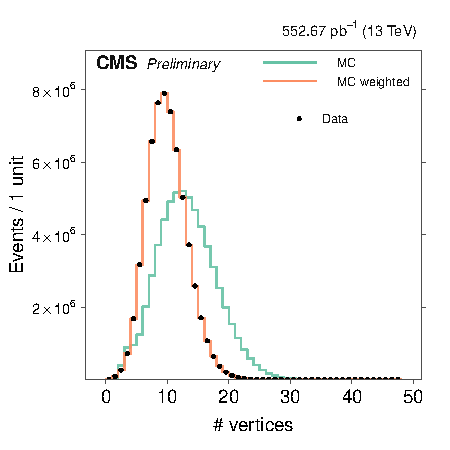
\includegraphics[scale=1.00]{figures/pileup_reweighting/f042_corr_nVert_data_mc_norm}
\caption{The distributions of the number of the reconstructed vertices
in the data, the simulated events, and the reweighted simulated events.
One is added to the the number of the reconstructed vertices.}
\label{f042_corr_nVert_data_mc_norm}
\end{figure}

The reweighting factors are derived as follows. First, we create the
distributions of the numbers of the reconstructed vertices for the data
and simulated sample. In creating these distributions, we add one to the
number of the reconstructed vertices. This is because these events do
not have the vertex for the main interaction while the events in the
signal and control regions do. Second, we smooth each distribution with
the smoothing spline. Third, we take the ratio of the two distributions,
i.e., the data over the simulated sample. The ratio is a function of the
number of reconstructed vertices. The ratio becomes reweighting factors
after normalised. The reweighting factors are normalised so as to
preserve the number of the generated events.

Figure~\ref{f042_corr_nVert_data_mc_norm} shows the distributions of the
number of the reconstructed vertices in the data, the simulated events,
and the reweighted simulated events. In the figure, one is added to the
the number of the reconstructed vertices. The figure demonstrates that
the reweighted simulated events have the distribution of the number of
the reconstructed vertices nearly identical to that in the data.


\subsection{Cross sections for SM samples}
Several MC samples of individual SM processes are binned according to a generator level quantity, such as the partonic \HT or bosonic \PT.
This analysis chooses to use samples binned in partonic \HT, for the set of MC samples (W+jets, DY+jets, QCD, $\gamma$+jets, $Z\rightarrow \nu\nu$+jets) and $\hat{P_{T}}$
for only the QCD sample.
These binned samples are provided with LO cross sections. The \kfactors required to go from LO to NNLO cross section are typically determined using corresponding
inclusive samples applied to each \HT binned sample.
Further studies can provide additional corrections to the cross sections, which can prove important to the closure test procedures described in
Section \ref{sec:closure-tests-desc}. As can be seen in Section \ref{sec:sideband_corrections}, residual cross section
corrections are measured using data in sidebands designed to enriched specific processes.

Following an inclusive selection, the distribution of the MC samples with respect to the binning variable $H_{T}^{parton}$ are shown in Fig.~\ref{fig:Lhe_Ht}, with
also the $\hat{P_{T}}$ distribution for QCD.

As stated above, the distributions shown in Fig.~\ref{fig:Lhe_Ht} follow an inclusive selection, whereby there is no requirement on each event. This direct translation
from MC allows to merge the binned generator level variable, and exhibits a smooth shape with respect to the cross sections in question.

A more in depth, data-driven investigation of the cross sections is shown in Sec.~\ref{sec:sideband_corrections}. Of which, an important point to note is that
the corrections to the cross sections, derived with the data sidebands are only relevant for data/MC comparison plots and the suite of closure tests defined in Section \ref{sec:closure-tests-desc}.

\begin{figure}[!h]
  \begin{center}
    \subfigure[$Z\rightarrow \nu\nu$ +jets] {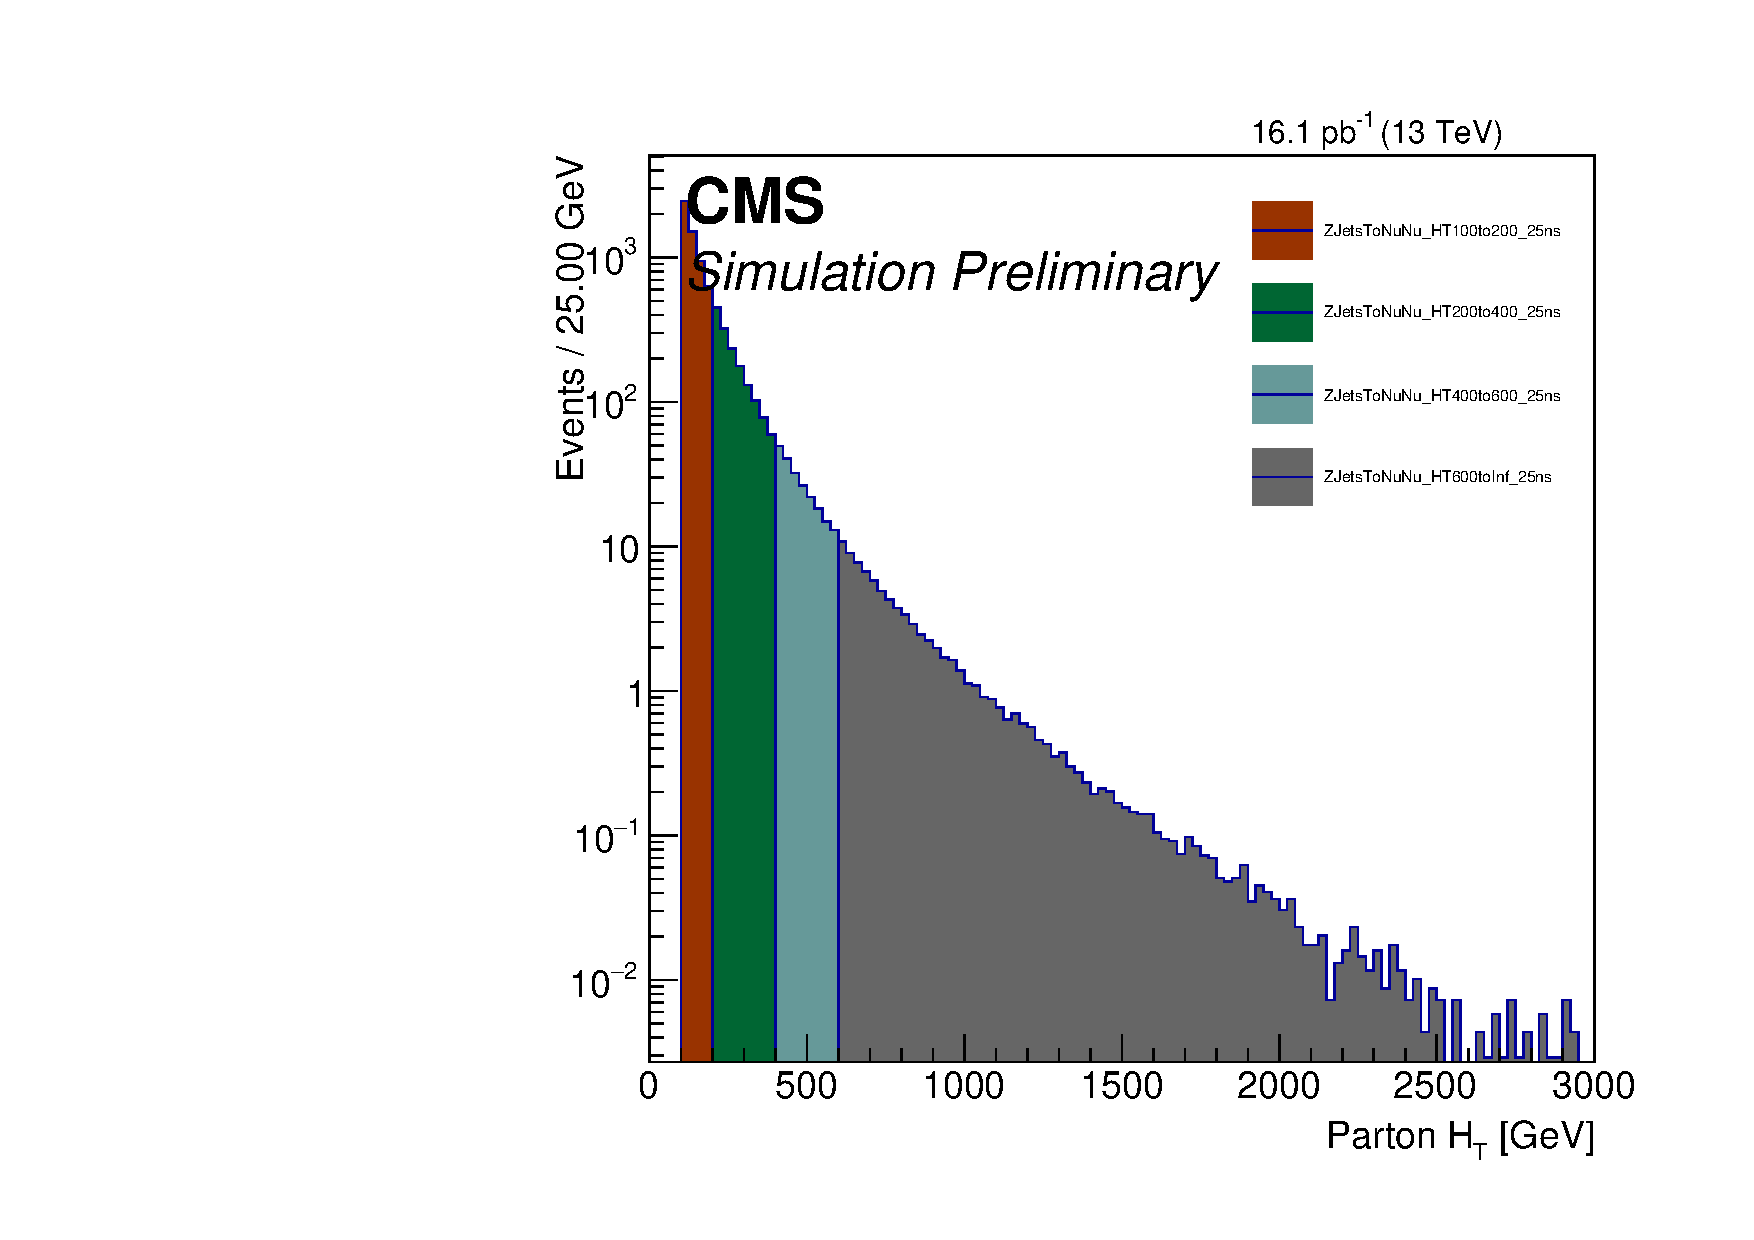
\includegraphics[width=0.45\textwidth]{figures/binnedMCsamples/Zinv.pdf}} ~~
    \subfigure[$W\rightarrow l \nu$ + jets]{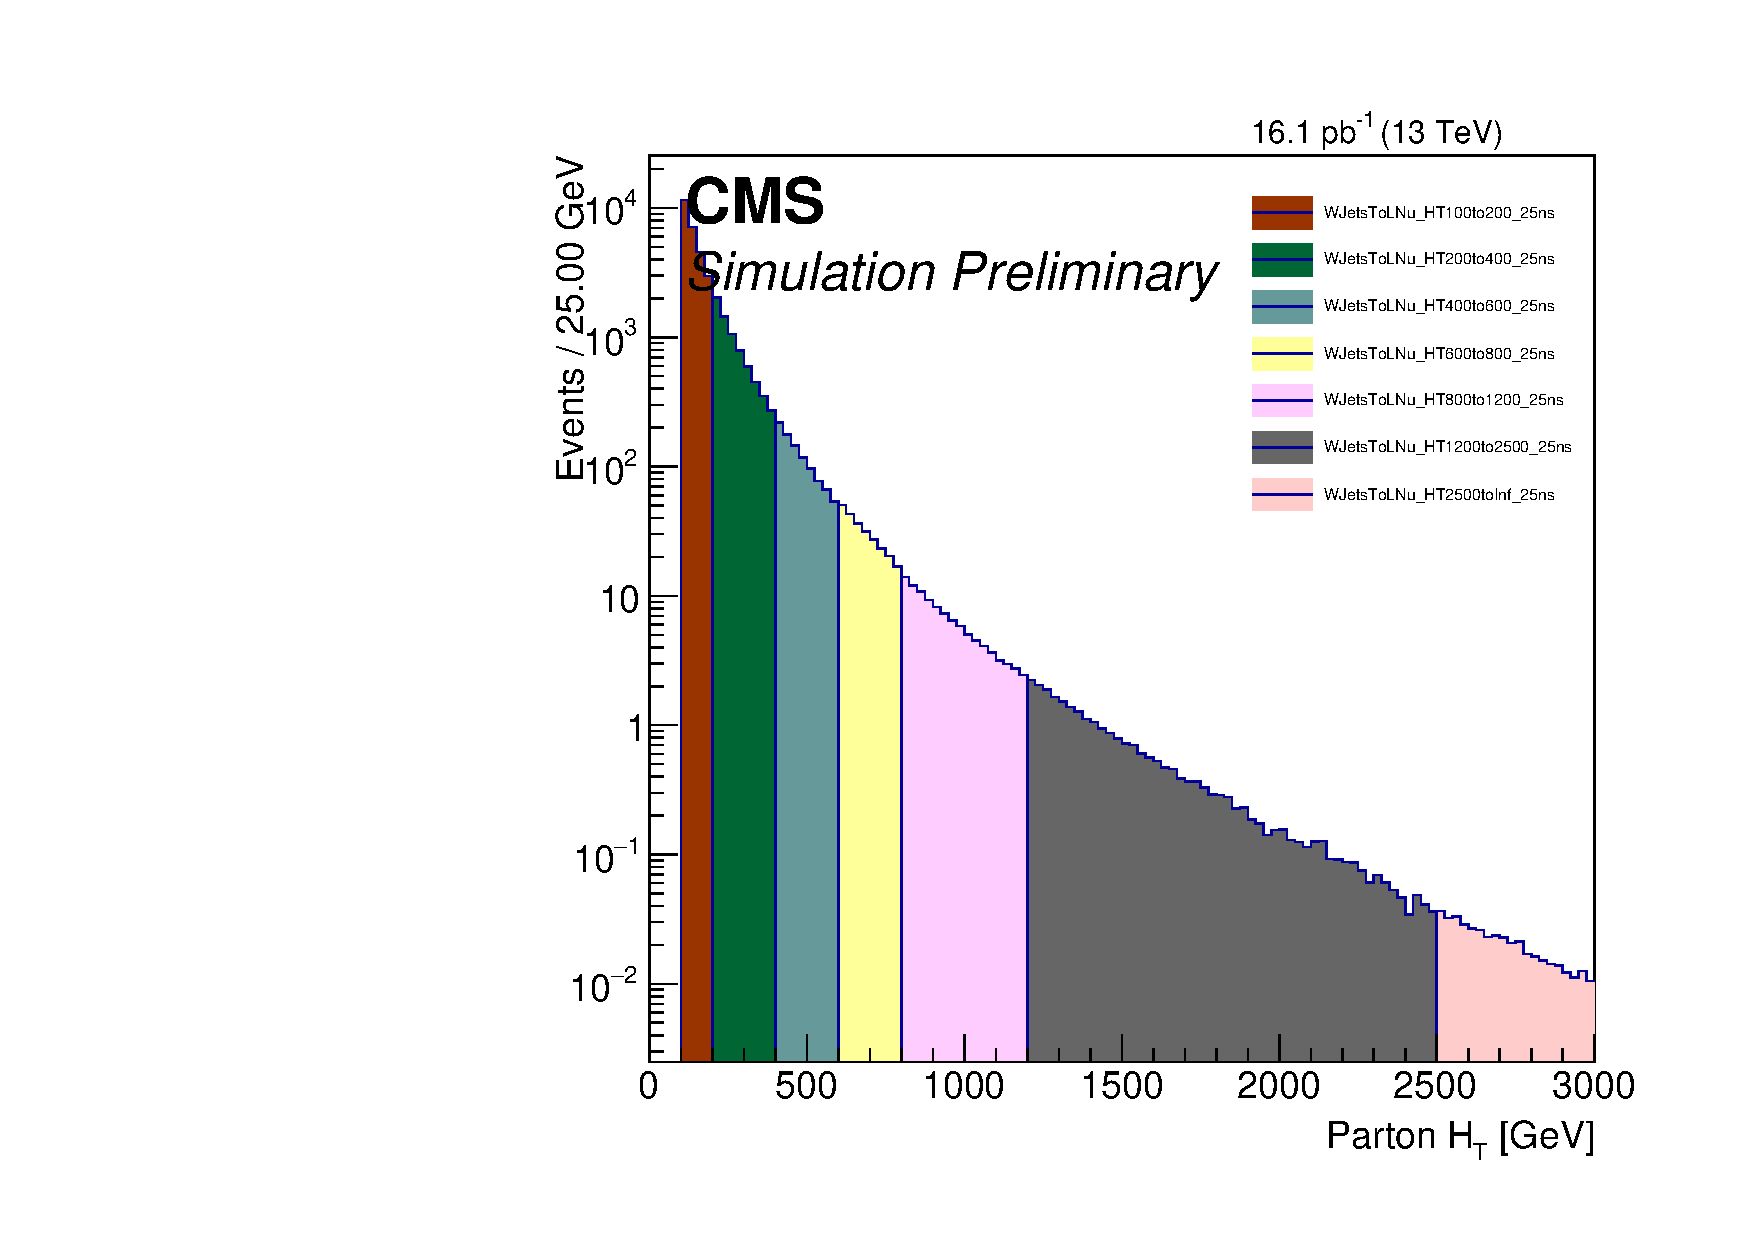
\includegraphics[width=0.45\textwidth]{figures/binnedMCsamples/WJetsToLNu_HT.pdf}} \\
    \subfigure[$DY\rightarrow ll$ + jets]{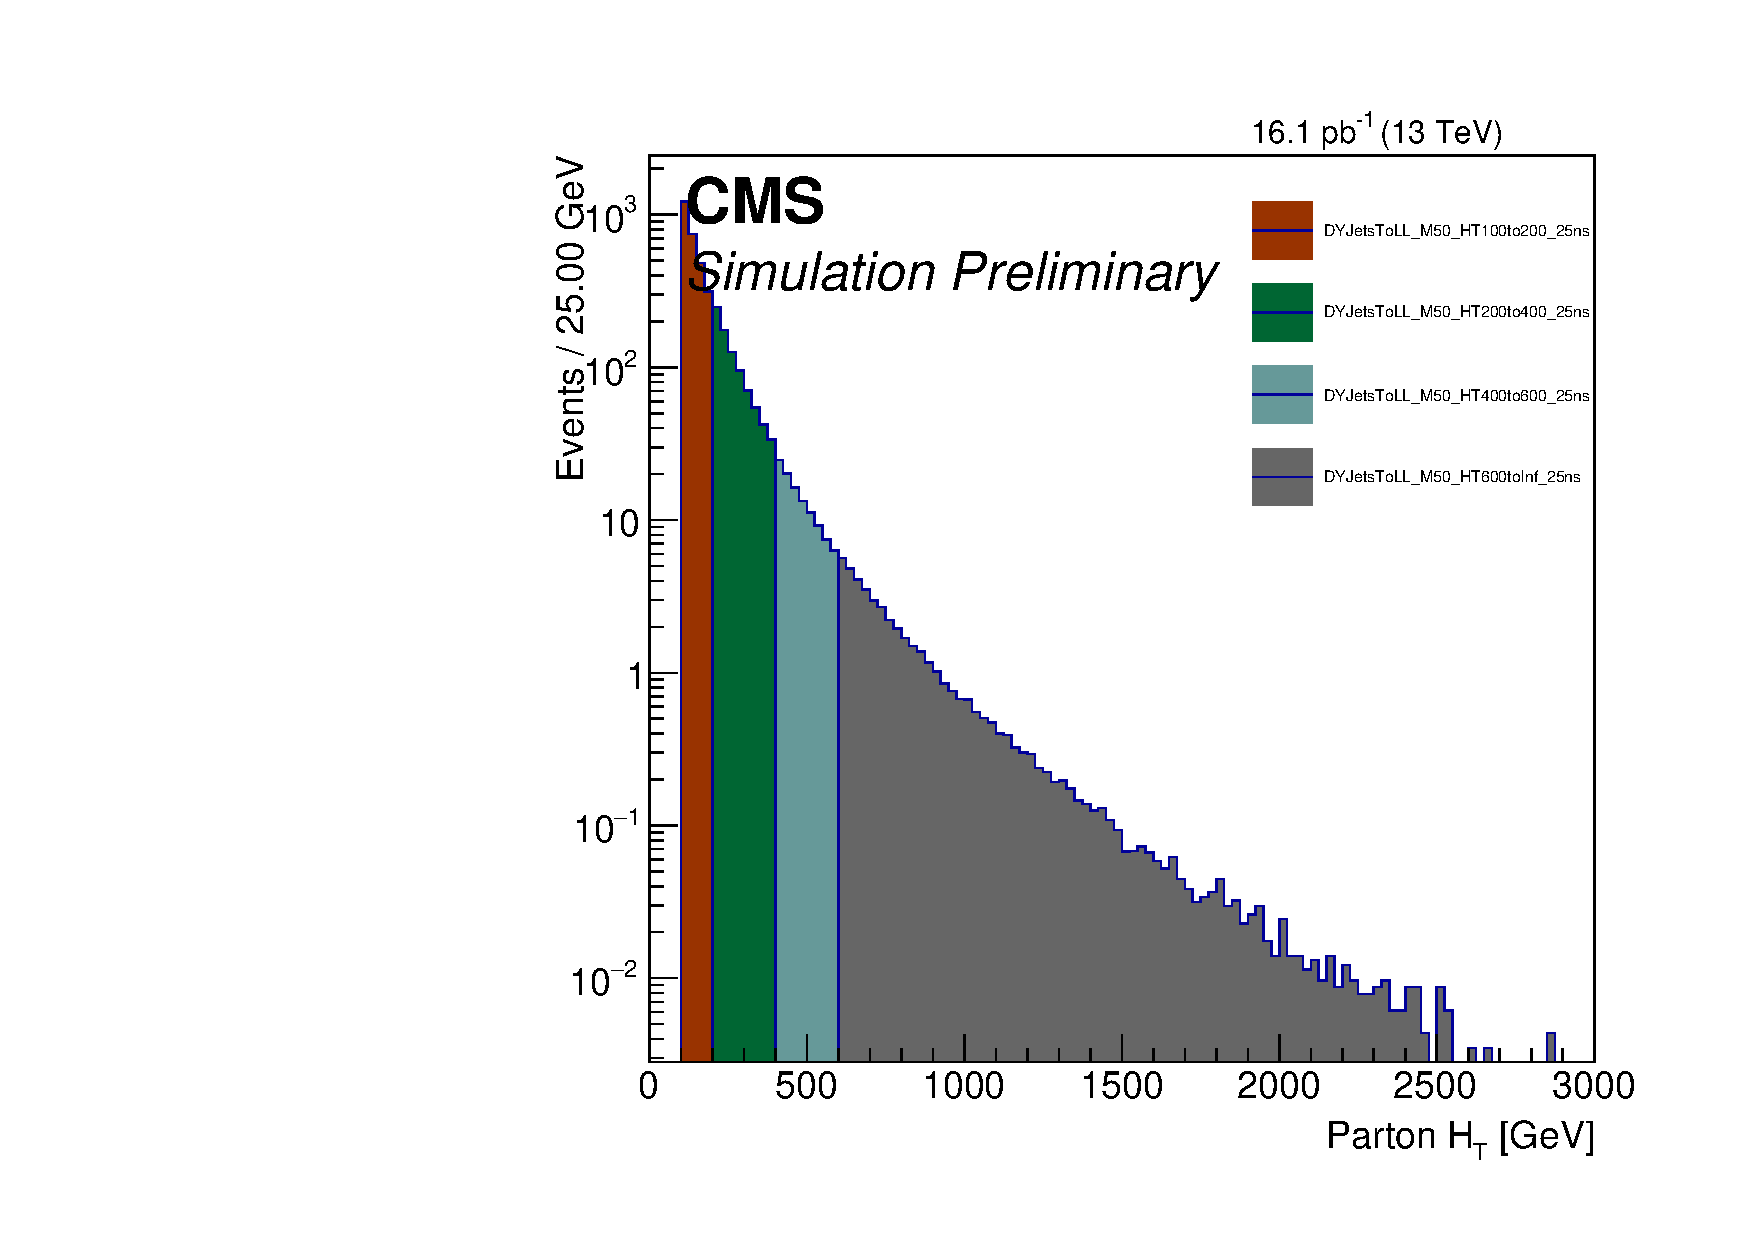
\includegraphics[width=0.45\textwidth]{figures/binnedMCsamples/DYJetsToLL_M50_HT.pdf}} ~~
    \subfigure[QCD]{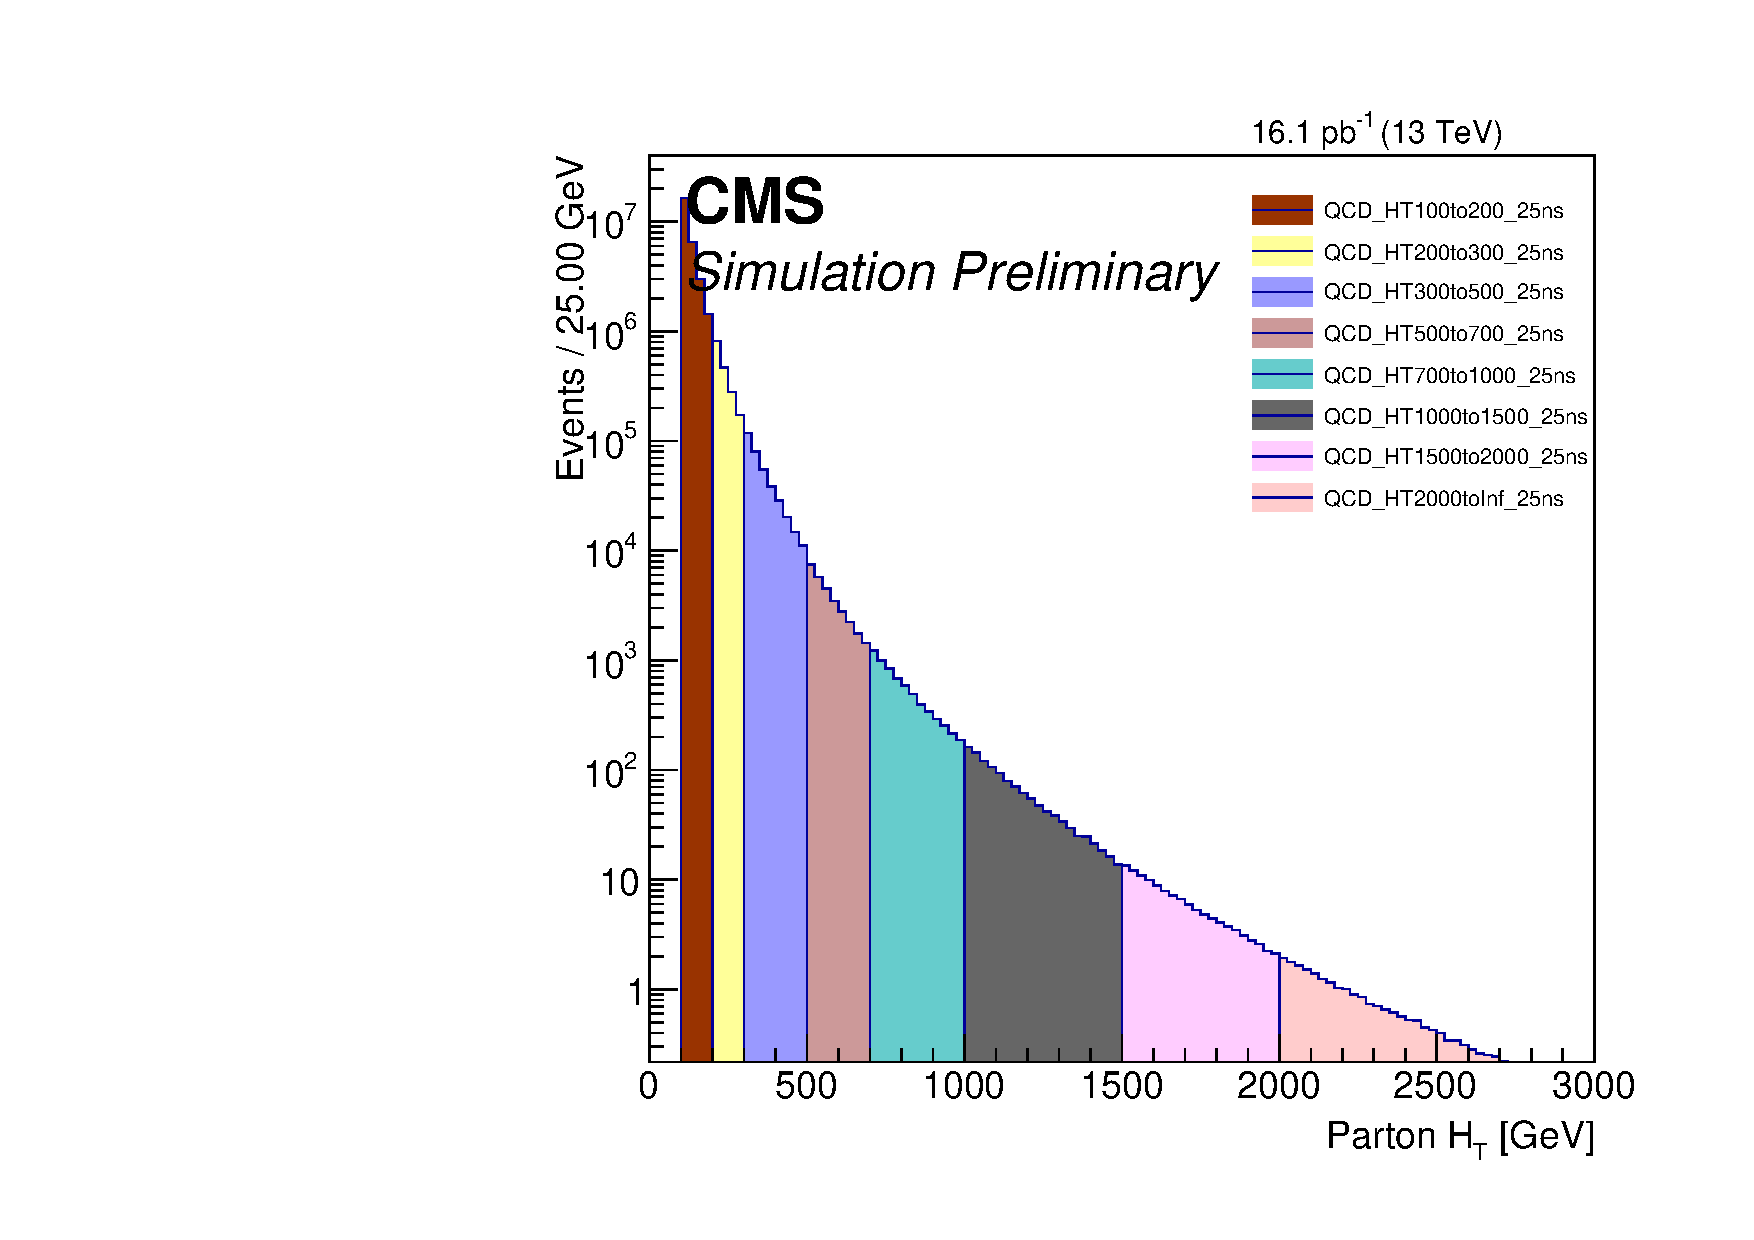
\includegraphics[width=0.45\textwidth]{figures/binnedMCsamples/QCD_HT.pdf}} \\
    \subfigure[$\gamma$+jets]{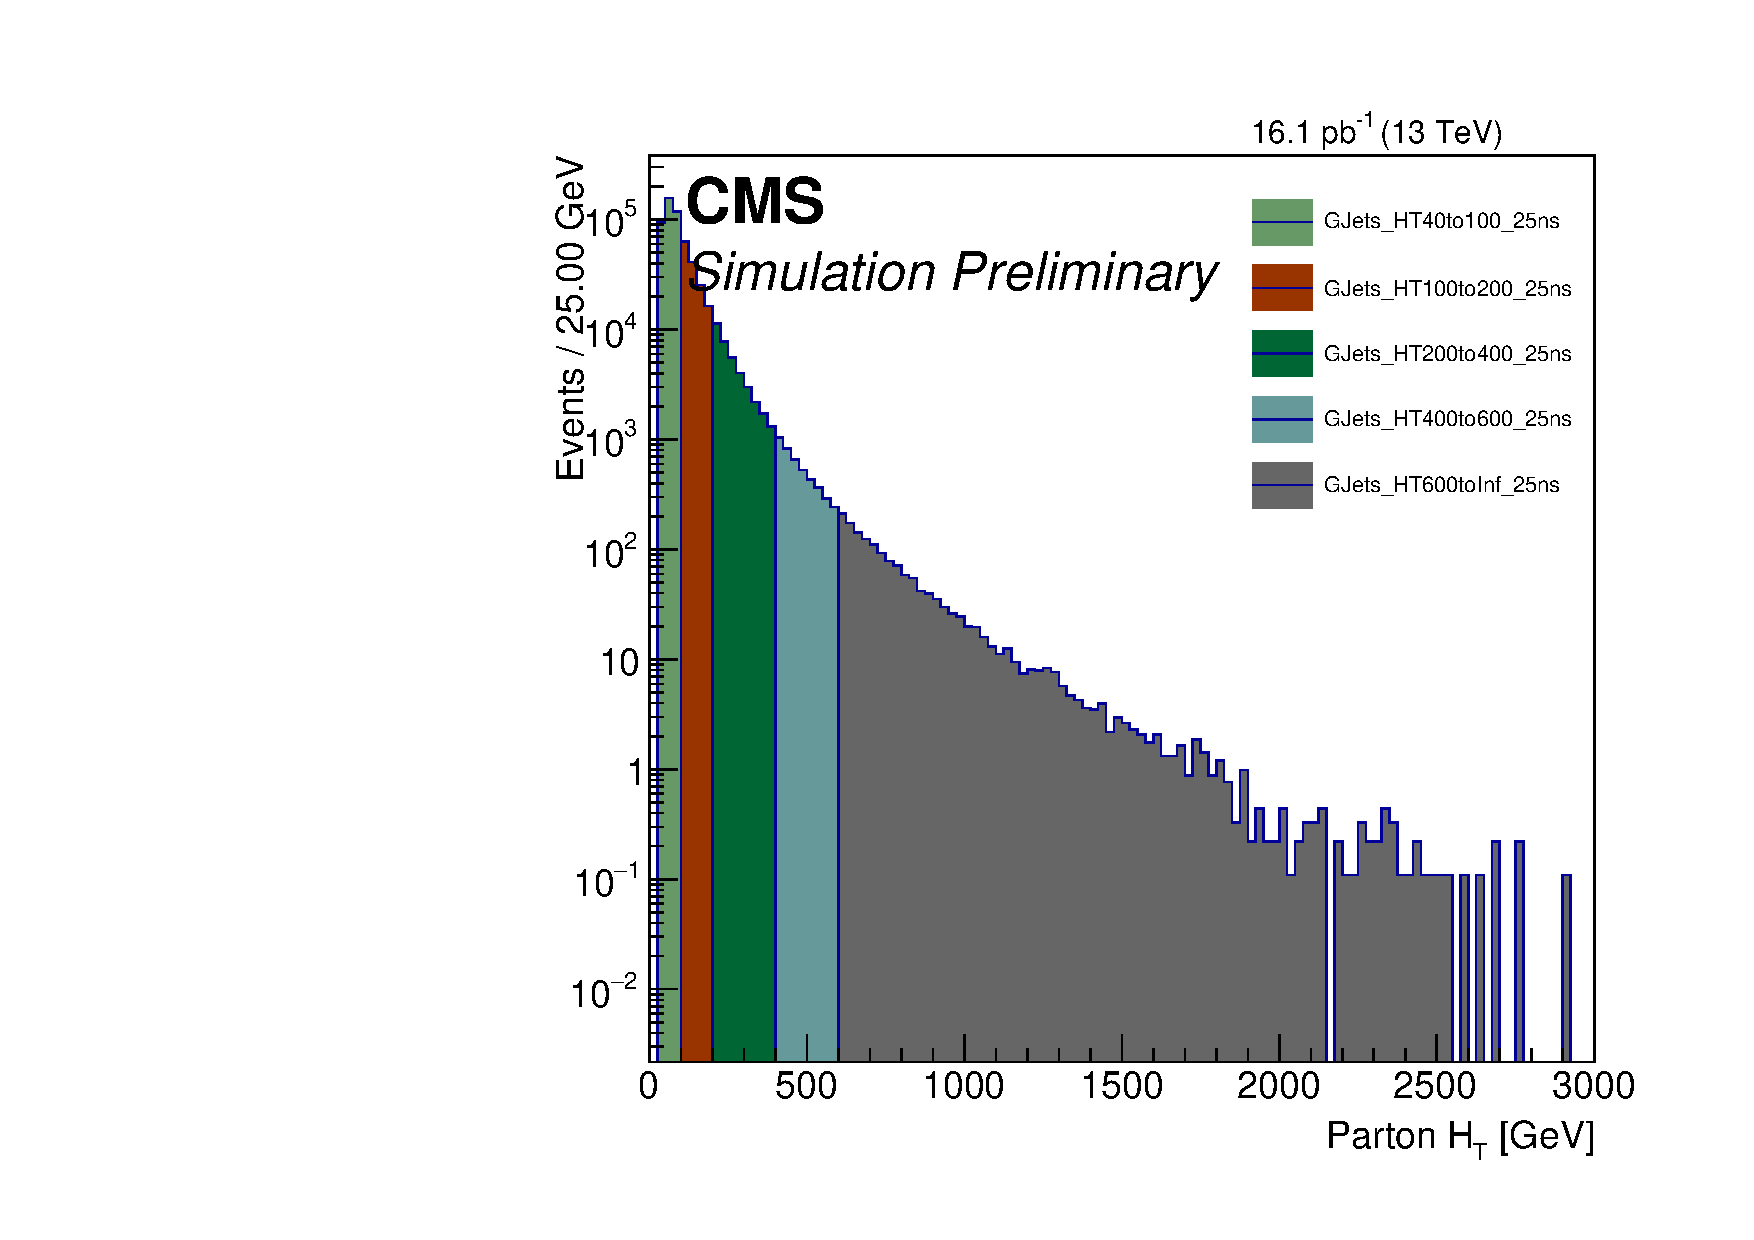
\includegraphics[width=0.45\textwidth]{figures/binnedMCsamples/GJets_HT.pdf}} ~~
    \subfigure[QCD $\hat{P_{T}}$]{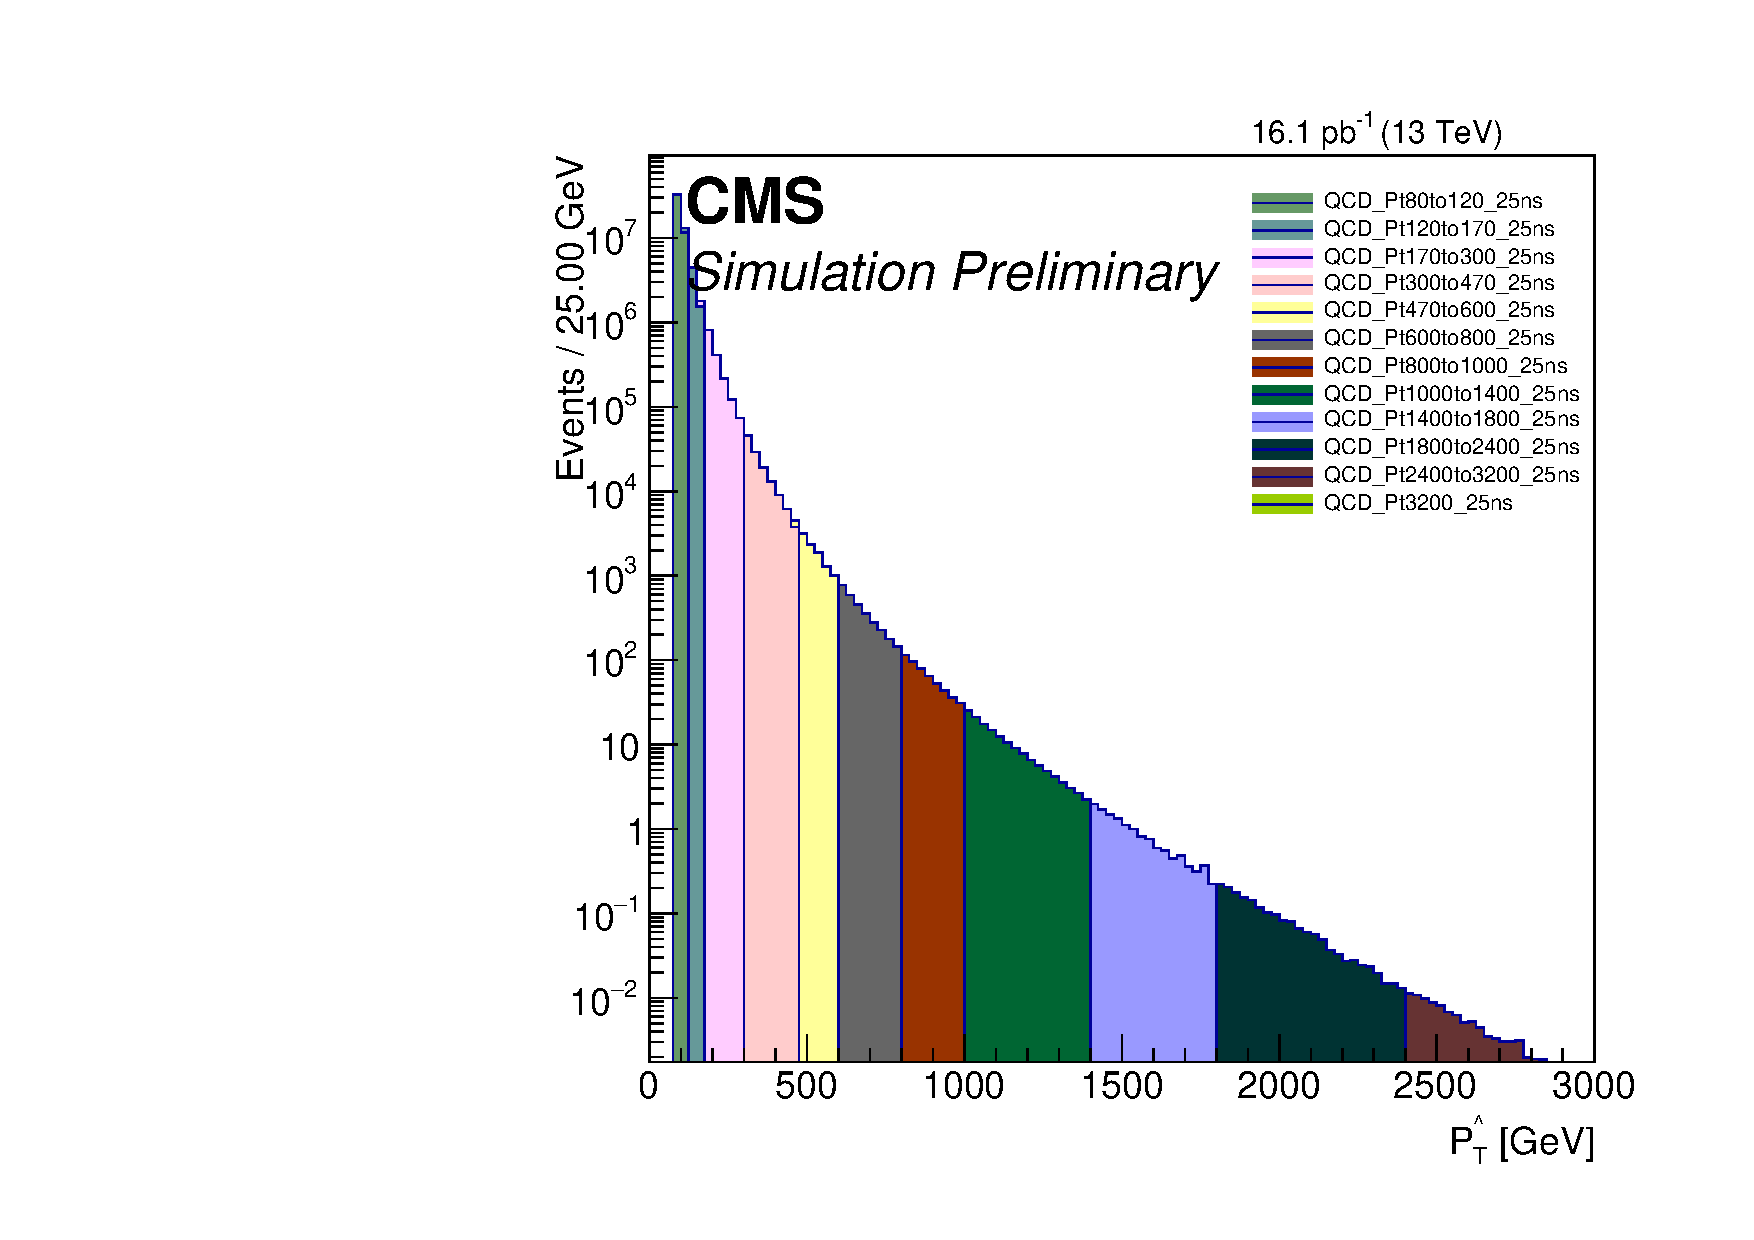
\includegraphics[width=0.45\textwidth]{figures/binnedMCsamples/QCD.pdf}}\\
    \caption{Generator-level $H_{T}^{parton}$ distributions for SM process, $Z\rightarrow \nu\nu$ + jets, W+jets, DY+jets, QCD, $\gamma$+jets, and $\hat{P_{T}}$ for QCD.}
    \label{fig:Lhe_Ht}
  \end{center}
\end{figure}

%%____________________________________________________________________________||
